% !TeX spellcheck=en_GB

\documentclass[a4paper,11pt]{article}

\usepackage{lnotes}

\DeclareGraphicsExtensions{.pdf,.eps,.png,.jpg}
\graphicspath{{./graphics/}}

\usetikzlibrary{decorations.markings}

\title{\boldmath Algebraic Topology}
\author{\href{https://github.com/rjm263}{rjm263}}
\email{}
\lecturer{\href{https://www.dpmms.cam.ac.uk/~jar60/}{Jacob Rasmussen}}
\term{Michealmas}
\a{2019}


\begin{document}
	
	\maketitle
	\flushbottom
	\newpage

	\section{Homotopy}
		
		\begin{defi}
			Let \(X,Y\) be topological spaces, \(f_0,f_1:X\rightarrow Y\) continuous maps 
			and \(I=[0,1]\). \(f_0\) is \textit{homotopic} to \(f_1\) if there is a continuous map 
			\(F:X\times I\rightarrow Y\) with 
			\begin{align}
			\forall x\in X: F(x,0)=f_0(x),\quad F(x,1)=f_1(x).
			\end{align}
			Denote by \(f_t(x)=F(x,t)\) the path from \(f_0\) to \(f_1\) in 
			\(\map(X,Y)=\{f:X\rightarrow Y|f\text{ continuous}\}\).
		\end{defi}
		Convention: all spaces are assumed to be topological and all maps to be continuous 
		for this course.
		\begin{eg}
			The following are all examples of homotopic maps:
			\begin{enumerate}
				\item \(f_0,f_1:\R^n\ra\R^m\) with \(f_1(0)=x\), i.e. \(f_0\sim f_1\) via 
				\(f_t(x)=t x\)
				\item \(S^1=\left\{ z\in\Co||z|=1\right\},\,f_0,f_1:S^1\ra S^1;\,f_0(z)=z,f_1(z)=-z\), then \(f_0\sim f_1\) via \(f_t(z)=\e{\ii\pi t}z\).
				\item \(S^n=\left\{ v\in\R^{n+1}|\norm{v}=1 \right\}\), \(f_0,f_1:S^n\ra S^n,\,f_0(v)=v,\,f_1(v)=-v\) (antipodal map)\\
				\(n=1:\,f_0\sim f_1,\\ n=2:\,f_0\nsim f_1.\)\\ In general, \(f_0\sim f_1\) iff $n$ is odd (see ES1 Q9)
				\item \(f_0,f_1: S^1\ra S^2\) where \(f_0(x,y)=(0,0,1),\,f_1(x,y)=(x,y,0)\), then \(f_0\sim f_1\) via \(f_t(x,y)=(tx,ty,\sqrt{1-t^2})\)
				\item \(D^n=\left\{ v\in R^n|\norm{v}\le1\right\}\) with \(S^{n-1}\subset D^n\). Say \(f:S^{n-1}\ra Y\) extends to \(D^n\) if there exists \(F:D^n\ra Y\) with \(F|_{S^{n-1}}=f\). $f$ extends to $D^n$ if and only if $f$ is homotopic to a constant map $f_t(v)=F(tv)$.
			\end{enumerate}
		\end{eg}
		\begin{lemma}
		Homotopy is an equivalence relation on $\map(X,Y)$ 
		\end{lemma}
		\begin{defi}
		Define 
		\begin{align*}
			[X,Y]=\map(X,Y)/\sim\,&=\left\{ \text{homotopy classes of maps }X\ra Y\right\}\\&=\left\{ \text{path components of }\map(X,Y)\right\}
		\end{align*}
		\end{defi}
		
		\begin{lemma}\label{lem--1.5}
		Suppose $f_0,f_1:X\ra Y$ and $g_0,g_1:Y\ra Z$. If $f_0\sim f_1$ and $g_0\sim g_1$ then $g_0\circ f_0\sim g_1\circ f_1$.
		\end{lemma}
		
		Notation: If $c\in Y$, $c_X:X\ra Y$ is given by $c_X(x)=c$ for all $x\in X$.
		
		\begin{cor}\label{cor--1.6}
			Any $f:X\ra\R^n$ is homotopic to $0_X$.
		\end{cor}
		\begin{proof}
			It is $\id_{\R^n}\sim 0_X$, so $f\sim\id_{\R^n}\circ f\sim 0_X\circ f=0_X$. 
		\end{proof}
		
		\begin{defi}\label{def--1.7}
			$X$ is \textit{contractible} if $\id_X\sim c_X$ for some $c\in X$.
		\end{defi}
		
		\begin{prop}
			$Y$ is contractible if and only if $[X,Y]$ has one element for all spaces $X$.
		\end{prop}
		\begin{proof}
			`$\Longrightarrow$': as in \autoref{cor--1.6}\\
			\phantom{\textit{Proof. }}`$\Longleftarrow$': $[X,Y]$ has one element, thus $\id_Y\sim c_Y$ for all $c\in Y$.
		\end{proof}
		
		\begin{defi}
			Spaces $X$ and $Y$ are said to be \textit{homotopic} $(X\sim Y)$ if there are maps $f:X\rightarrow Y$ and $g:Y\rightarrow X$ such that $f \circ g\sim\id_{Y}$ and $g \circ f\sim\id_{X}$.
		\end{defi}

		\begin{remark}
			If spaces $X,Y$ are homeomorphic, then they are also homotopic. However, the converse is not true in general.
		\end{remark}
		
		\begin{eg}\label{ex--contractible}
			$X\sim \left\{ p\right\}$ if and only if $X$ is contractible.
		\end{eg}
		\begin{proof}
			Consider $f:X\rightarrow \left\{ p\right\}, x\mapsto p$ and $g:\{p\} \rightarrow X,p\mapsto c\in X$. Then $f \circ g=\id_{\{p\}}$ and $g \circ f=c_{X}$. But if $X$ is contractible, then $g \circ f\sim\id_{X}$. Hence,
			\begin{equation}
				c_{X}\sim\id_{X}\Longleftrightarrow X\text{ is contractible}
			\end{equation}
			according to \autoref{def--1.7}.
		\end{proof}
		
		\begin{lemma}
			If $X_1\sim X_2$ and $Y_1\sim Y_2$ then there is a bijection $[X_1,Y_1]\simeq [X_2,Y_2]$.
		\end{lemma}

		Now having developed the notion of homotopy between maps and spaces and what it means for a space to be contractible, one can ask the basic question: given spaces $X,Y$, are they homotopic? And if so, what is $[X,Y]$? The answer to these questions are to be found in the homotopy groups introduced in the following.

		\subsection{Homotopy Groups}
			
			\begin{defi}(Maps of Pairs)
				The map $f:(X,A)\rightarrow (Y,B)$ means
				\begin{enumerate}
					\item $A\subset X,B\subset Y$
					\item $f:X\rightarrow Y$
					\item $f(A)\subset B$
				\end{enumerate}
				If $f_0,f_1:(X,A)\rightarrow (Y,B)$, we say $f_0\sim f_1$ if
				\begin{equation}
					\exists F:(X\times I,A\times I)\rightarrow (Y,B):\,F(x,0)=f_0(x),F(x,1)=f_1(x).
				\end{equation}
			\end{defi}

			Notation: $\ast=(-1,0,\dots,0)\in S^{n}$.

			\begin{defi}
				If $p\in X$, we define the \textit{nth homotopy group} as
				\begin{equation}
					\pi_{n}(X,p)=[(S^{n},\ast),(X,p)]=[(D^{n},S^{n-1}),(X,p)]=[(I^{n},\partial I^{n}),(X,p)].
				\end{equation}
				We denote with $\pi$ the map
				\begin{equation}
					\pi:D^{n}\rightarrow D^{n}/S^{n-1}\simeq S^{n},\quad v\mapsto(1-2\norm{v},v\cdot\alpha(v)),
				\end{equation}
				where $\alpha(v)=\sqrt{1-(1-2\norm{v})^2}$.
			\end{defi}
			From the above definition of homotopy groups follow the 
			\begin{pro}\phantom{kk}
				\begin{itemize}
					\item $n>0$: $\pi_n(X,p)$ is a group: e.g. $n=2$\\
					group operation: 
					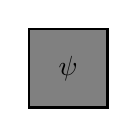
\begin{tikzpicture}[baseline=.3cm]	
						\draw[fill=gray,thick] (0,0) rectangle (1,1);\node at (.5,.5){$\psi$};
					\end{tikzpicture} $+$ \tikz[baseline=.3cm]{\draw[thick] (0,0) rectangle (1,1);\node at (.5,.5){$\varphi$};} $=$ \tikz[baseline=.3cm]{\draw[fill=gray,thick] (0,0) rectangle (1,1);\node at (.5,.5){$\psi$};\draw[thick] (1,0) rectangle (2,1);\node at (1.5,.5){$\varphi$}}\\
					identity element: \tikz[baseline=.3cm]	
					{\draw[fill=lightgray,thick] (0,0) rectangle (1,1)} $+$ \tikz[baseline=.3cm]{\draw[thick] (0,0) rectangle (1,1);\node at (.5,.5){$\varphi$};} $=$ \tikz[baseline=.3cm]{\draw[fill=lightgray,thick] (0,0) rectangle (1,1);\draw[thick] (1,0) rectangle (2,1);\node at (1.5,.5){$\varphi$}} $\sim$ \tikz[baseline=.3cm]{\draw[thick] (0,0) rectangle (1,1);\node at (.5,.5){$\varphi$}}, with \tikz[baseline=.3cm]{\draw[fill=lightgray] (0,0) rectangle (1,1)} the constant map $I^n\rightarrow p$ (this also applies to the next picture).
					
					\item $n>1$: $\pi_{n}(X,p)$ is abelian:\\ $\psi+\varphi=$ \tikz[baseline=.3cm]{\draw[thick] (0,0) rectangle (1,1);\draw[thick] (1,0) rectangle (2,1);\node at (.5,.5){$\psi$};\node at (1.5,.5){$\varphi$}} $\sim$ \tikz[baseline=.7cm]{\draw[fill=lightgray,thick] (0,0) rectangle (2.5,2);\draw[fill=white,thick] (.3,.5) rectangle (1.1,1.3);\draw[fill=white,thick] (1.4,.5) rectangle (2.2,1.3);\node at (.7,.9){$\psi$};\node at (1.8,.9){$\varphi$};
					\draw[<-,thick] (1.8,1.5) arc [radius=1, start angle=55, end angle=125];\draw[->,thick] (1.8,.3) arc [radius=1, start angle=305, end angle=235]} $\sim$ \tikz[baseline=.7cm]{\draw[fill=lightgray,thick] (0,0) rectangle (2.5,2);\draw[fill=white,thick] (.3,.5) rectangle (1.1,1.3);\draw[fill=white,thick] (1.4,.5) rectangle (2.2,1.3);\node at (.7,.9){$\varphi$};\node at (1.8,.9){$\psi$}} $\sim\varphi+\psi$
					
					\item \textit{induced maps}: $f:(X,p)\rightarrow (Y,q)$ induces $f_{\ast}:\pi_{n}(X,p)\rightarrow \pi_{n}(Y,q)$ with $f_{\ast}([\gamma])=[f \circ \gamma]$ well defined by \autoref{lem--1.5}. They satisfy the following properties:
					\begin{enumerate}
						\item $(\id_{(X,p)})_{\ast}=\id_{\pi_{n}(X,p)}$,
						\item $(f \circ g)_{\ast}=f_{\ast} \circ g_{\ast}$.
					\end{enumerate}
					Note also that $f_{\ast}$ is homotopy invariant: if $f\sim g$, then $f_\ast=g_\ast$ since $f_\ast([\gamma])=[f \circ \gamma]=[g\circ \gamma]=g_{\ast}([\gamma])$.
					\item this defines a functor
						\begin{align*}
						\begin{Bmatrix}
							\text{pointed spaces}\\\text{pointed maps}
						\end{Bmatrix}
						\quad&\longrightarrow\quad 
						\begin{Bmatrix}
							\text{groups}\\ \text{homomorphisms}
						\end{Bmatrix}\\
						X\quad&\xmapsto{\phantom{kkl}}\quad \pi_{n}(X,p)\\
						f:(X,p)\rightarrow (Y,q)\quad&\xmapsto{\phantom{kkl}} \quad f_{\ast}:\pi_{n}(X,p)\rightarrow \pi_{n}(Y,q) 
						\end{align*}
				\end{itemize}
			\end{pro}


	\section{Homology}

		The goal here is to define functors
		\begin{align*}
			\begin{Bmatrix}
				\text{topological spaces}\\ \text{continuous groups}
			\end{Bmatrix}
			\quad&\longrightarrow \quad
			\begin{Bmatrix}
				\text{abelian groups}\\\text{homomorphisms}
			\end{Bmatrix}\\
			X\quad&\xmapsto{\phantom{kkl}}\quad H_{n}(X)\\
			f:X\rightarrow Y\quad&\xmapsto{\phantom{kkl}}\quad f_{\ast}:H_{n}(X)\rightarrow H_{n}(Y)
		\end{align*}
		such that the following are satisfied:
		\begin{enumerate}
			\item $(\id_{X})_{\ast}=\id_{H_{n}(X)}$
			\item $(f \circ g)_{\ast}=f_{\ast}\circ g_{\ast}$
			\item if $f\sim g$, then $f_{\ast}=g_{\ast}$
			\item $H_n(X)=0$ if $n>\dim X$ (dimension axiom)	
		\end{enumerate}


		\subsection{Chain Complex}
			Let $R$ be a commutative ring (e.g. $\Z,\Q,Z/p$).

			\begin{defi}
				A chain complex $(C_\ast,d)$ over $R$ is
				\begin{enumerate}
					\item $R$-modules $C_i$ for $i\in\Z$ and
					\item homomorphisms $d_i:C_i \rightarrow C_{i+1}$ such that
					\item $d_i \circ d_{i+1}=0$ for all $i\in\Z$.
				\end{enumerate}
				\begin{tikzcd}
				 \phantom{A}\dots\arrow[r]& C_{i+1}\arrow[r,"d_{i+1}"] & C_i\arrow[r,"d_i"] & C_{i-1}\arrow[r]&\dots\phantom{B}
				\end{tikzcd}
			\end{defi}
			Notation: $C_\ast$ can either mean $\ast$ is $i\in\Z$ or $C_\ast=\bigoplus_{i\in\Z}C_i$ with $d=\sum d_i$ where $d:C_\ast \rightarrow C_{\ast -1}$. In this notation (iii) in the definition above becomes $d^2=0$.

			\begin{defi}(Simplex)
				Define \begin{equation}
					\Delta^{n}=\{ v=(v_0,\dots,v_n)\in\R^{n+1}|v_i\ge 0,\sum_iv_i=1\}
				\end{equation}
				to be the \textit{n-dimensional simplex}.
			\end{defi}

			\begin{eg}
				It is $\Delta^{-1}=\emptyset$, and\\ $n=0$: \ \ 
				
\begin{tikzpicture}
					\draw [fill] (0,0.5) circle [radius=.08];
				\end{tikzpicture}
				\ \ , $n=1$:
				\begin{tikzpicture}[baseline=.3cm]
					\draw[thick] (0,1) -- (1,0);
					\draw[dotted] (0,-.3) -- (0,1.3);
					\draw[dotted] (-.3,0) -- (1.3,0);
				\end{tikzpicture}
				\ \ , $n=2$:
				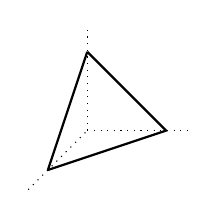
\begin{tikzpicture}[baseline=.1cm]
					\draw[dotted] (-.75,-.75) -- (0,0);
					\draw[dotted] (0,0) -- (0,1.3);
					\draw[dotted] (0,0) -- (1.3,0);
					\draw[thick] (-.5,-.5) -- (1,0) -- (0,1);
					\draw[thick] (-.5,-.5) -- (0,1);
				\end{tikzpicture}
				\ \ \hspace{1cm}etc.
			\end{eg}

			\begin{defi}(Faces)
				If $I=\{i_0<i_1<\dots<i_k\}\subset \{0,1,\dots,n\}$, then \begin{equation}
					f_I=\{v\in\Delta^{n}|v_i=0\text{ if }i\notin I\}
				\end{equation} is a \textit{k-dimensional face} of $\Delta^{n}$.
			\end{defi}

			\begin{defi}(Face maps)
				Maps \begin{equation}
					F_I:\Delta^{k}\rightarrow f_I,\quad w\mapsto v,\quad v_i=\begin{cases}
						0, & i\notin I\\w_j, & i=\varphi(j)
					\end{cases},
				\end{equation}
				where $\varphi:\{0,\dots,k\}\rightarrow I,\,\varphi(j)=i_j$.
			\end{defi}

			\begin{defi}(reduced chain complex of a simplex)\label{def--2.6}
				The \textit{reduced chain complex} over $\R$ is defined by $\tilde{S}_k (\Delta^{n})=\langle f_I||I|=k+1\rangle$ free abelian group with basis the k-dimensional faces $f_I$. We also have
				\begin{equation}
					d_{k}:\tilde{S}_{k}(\Delta^{n})\rightarrow\tilde{S}_{k-1}(\Delta^{n}),\quad d_{k}(f_I)=\sum_{j=0}^{k}(-1)^{j}f_{I\backslash\{i_j\}}. 
				\end{equation}
			\end{defi}

			\begin{eg}($n=2$)
				\begin{equation*}
					\begin{tikzcd}[row sep=tiny]
					C_2\ar[d,equal]\arrow[r]& C_1\ar[d,equal]\arrow[r]& C_0\ar[d,equal]\arrow[r]& C_{-1}\ar[d,equal]
					\\
					\langle f_{012}\rangle& \langle f_{01},f_{12},f_{02}\rangle& \langle f_{0},f_1,f_2\rangle& \langle f_{\emptyset}\rangle 
					\end{tikzcd}
				\end{equation*}
				We have \begin{align*}
					df_{012}=f_{12}-f_{02}+f_{01},\quad
					df_{12}=f_{2}-f_{1},\quad f_{02}=f_{0}-f_{2},\quad df_{01}=f_{0}-f_{1}
				\end{align*}
				and hence $d^2f_{012}=0$.
			\end{eg}

			\begin{prop}
				$d^2=0$ for the chain complex.
			\end{prop}
			\begin{proof}
				It is enough to show the above for an arbitrary face, $d^2f_I=0$. In order to show this, we use \autoref{def--2.6}:
				\begin{align}
					d^2f_I&=d\sum_i(-1)^i f_{I\backslash\{i\}}\\
					&=\sum_{\substack{i,j\\j<i}}(-1)^i(-1)^jf_{I\backslash\{j,i\}}+\sum_{\substack{i,j\\j>i}}(-1)^i(-1)^{j-1}f_{I\backslash\{i,j\}}\\
					&=\sum_{\substack{i,j\\j<i}}(-1)^i(-1)^jf_{I\backslash\{j,i\}}-\sum_{\substack{i,j\\j<i}}(-1)^i(-1)^{j}f_{I\backslash\{i,j\}}\\
					&=0
				\end{align}
			\end{proof}
			This property of the homomorphisms $d$ is crucial to the definition of homology on a space. Note that $d^2=0$ immediately implies $\im d_{i+1}\subset\ker d_{i}$. We make use of this in the following definition.

			\begin{defi}(Homology groups)
				If $(C_\ast,d)$ is a chain complex, it's \textit{ith homology group} is defined as \begin{equation*}
					H_{i}(C_{\ast})=\frac{\ker d_{i}}{\im d_{i+1}}
				\end{equation*}
				and again we abuse notation to denote with $\ast$ either of the two expressions
				\begin{equation*}
					H_{\ast}(C_{\ast})=\bigoplus_{i\in\Z}H_{i},\qquad H_{\ast}(C_{\ast})=\frac{\ker d}{\im d}.
				\end{equation*}
			\end{defi}

			\begin{eg}(Unreduced complex of a simplex)
				\begin{equation*}
					\text{Define }S_{k}(\Delta^{n})=\begin{cases}
						\tilde{S}_k(\Delta^{n}), & k\ge0\\ 0, & k<0
					\end{cases},\text{ can check that }H_{k}(S(\Delta^{n}))=\begin{cases}
						\Z, & k=0\\ 0, & k\neq 0
					\end{cases}
				\end{equation*}
			\end{eg}

			\begin{defi}(Chain maps)
				If $(C,d)$ and $(C ^{\prime},d ^{\prime})$ are chain complexes over $R$, a chain map $f:(C,d)\rightarrow (C ^{\prime},d ^{\prime})$ are homomorphisms $f_i:C_i \rightarrow C_i ^{\prime}$ such that all squares of the following diagram commute:
				\begin{equation*}
					\begin{tikzcd}
						\phantom{A}\dots\ar[r] & C_{i+1}\ar[d,"f_{i+1}"]\ar[r,"d_{i+1}"] & C_i\ar[d,"f_i"]\ar[r,"d_{i}"] & C_{i-1}\ar[d,"f_{i-1}"]\ar[r]&\dots\phantom{A}\\
						\phantom{A}\dots\ar[r] & C_{i+1}^{\prime}\ar[r] & C_{i}^{\prime}\ar[r] & C_{i-1}^{\prime}\ar[r] &\dots\phantom{A}
					\end{tikzcd}
				\end{equation*}
				i.e. $d ^{\prime}f=fd$ where $f=\sum f_i:C_\ast \rightarrow C_\ast ^{\prime}$.
			\end{defi}

			\begin{eg}
				If $f_I$ is a face of $\Delta^{n}$, there is a chain map $\phi_I:\tilde{S}_\ast(\Delta^{n})\rightarrow \tilde{S}_\ast(\Delta^{n})$ with $\phi_I(f_J)=f_{\varphi(J)}$.

				If $f:(C,d)\rightarrow (C ^{\prime},d ^{\prime})$ is a chain map, then 
				\begin{align*}
					d z=0\quad\Longrightarrow\quad d ^{\prime}fz=fdz=0\quad\Longrightarrow\quad f(\ker d)\subset\ker d ^{\prime},\\
					z=d y\quad\Longrightarrow\quad fz=fdy=d ^{\prime}fy\quad\Longrightarrow\quad f(\im d)\subset \im d ^{\prime}.				
				\end{align*}
				So there is a well-defined map $f_\ast:H_\ast(C)\rightarrow H_\ast(C ^{\prime}),\,[z]\mapsto[fz]$.
			\end{eg}
			Notation: If $dx=0$, write $[x]$ for the image of $x$ in $H_\ast(C)$.

			\begin{lemma}\phantom{j}
				\begin{enumerate}
					\item $\id_C$ is a chain map and $(\id_C)_\ast=\id_{H_\ast(C)}$
					\item if $f:C \rightarrow C ^{\prime}$ and $g:C ^{\prime}\rightarrow C^{\prime\prime}$ are chain maps, then so is $g\circ f$ and $(g \circ f)_\ast=g_\ast \circ g_\ast$	
				\end{enumerate}
				i.e. there is a functor 
				\begin{align*}
					H_\ast:\begin{Bmatrix}
						\text{\normalfont chain complexes over }R\\\text{\normalfont chain maps}
					\end{Bmatrix}
					\quad&\longrightarrow\quad
					\begin{Bmatrix}
						R\text{\normalfont\ modules}\\\text{\normalfont homomorphisms}
					\end{Bmatrix}\\
					(C,d)\quad&\xmapsto{\phantom{kkl}}\quad H_\ast(C)\\
					f:C \rightarrow C ^{\prime}\quad&\xmapsto{\phantom{kkl}}\quad f_\ast:H_\ast(C)\rightarrow H_\ast(C ^{\prime})
				\end{align*}
			\end{lemma}

		
		\subsection{Singular Chain Complex}

			The (simplicial) simplices $\Delta^n$ introduced above provide (to some extent) a good geometrical intuition about how a chain complex looks like. On the other hand, however, contructing a given space as a chain complex requires, e.g., a triangulation of the space and proof that the homology is independent of our choice of triangulation. This can be quite laborious already for relatively simple space.
			
			Luckily, there are other types of chain complexes and below we introduce the singular chain complex. The most notable advantage of this definition is that there is no triangulation business involved. As such, singular homology is manifestly a property of just the space itself. On the downside, a singular chain complex does not, i.g., consist of a finite number of simplices but can entail an infinite number (not necessarily countable) of singular simplices. Hence, they are monstrous and it is hopeless to try imagine how these chain complexes look like, let alone use it to compute the homology. However, it turns out that the definition is quite powerful in that, knowing the homology of some simple spaces, we can use it to compute homology groups of more complicated ones indirectly. This, however, requires us to do some groundwork first.
			
			\begin{defi}(Singular chain complex)
				Let $X$ be a topological space. A \textit{singular k-simplex} in $X$ is a map $\sigma:\Delta^{k}\rightarrow X$.
			\end{defi}

			\begin{defi}
				The singular chain complex $C_\ast(X)$ is given by
				\begin{align*}
					C_k(X)&=\langle\sigma|\sigma:\Delta^{k}\rightarrow X\text{ continuous}\rangle\\
					&=\text{ free abelian group generated by }\sigma 's.
				\end{align*}
			\end{defi}

			\begin{remark}
				Note that we can view an abelian group like $C_k(X)$ above as a $\Z$-module (for $\sigma\in C_k(X)$ write $\sigma+\dots+\sigma=n\sigma$).
			\end{remark}

			The elements of $C_k(X)$ are finite sums $\sum_{i=1}^{N}a_i\sigma_i,\,a_i\in\Z$ and the boundary homomorphisms act on these as
			\begin{equation}
				d(\sigma)=\sum_{i=0}^{k}(-1)^i\sigma \circ F_{\{0,\dots,k\}\backslash\{i\}}
			\end{equation} 
			with face maps $F_{\{0,\dots,k\}\backslash\{i\}}:\Delta^{k-1}\rightarrow \Delta^{k}$,\\ 
			e.g. $k=1$: \tikz[baseline=.3cm]{\draw[fill,thick] (0,0) circle [radius=.05];\draw[fill,thick] (.5,1.5) circle [radius=.05];\node [below] at (0,0) {$\tau_0$};\node [above] at (.5,1.5) {$\tau_1$};\draw[thick] (0,0) to [out=0,in=0] (.3,.7) to [out=180,in=180] (.6,.3) to [out=0,in=0] (.5,1.5)} $\mathrm{d}\sigma=\tau_1-\tau_0$, $\qquad k=2$: \tikz[baseline=.3cm,decoration={markings,mark=at position 0.5 with {\arrow{>}}}]{\draw[baseline=.3cm,fill=lightgray,lightgray] (0,0) to [out=20,in=300] (.6,1.5) to [out=340,in=60] (1.5,0) to [out=180,in=20] (0,0);\draw[postaction={decorate},thick] (0,0) to [out=20,in=300] (.6,1.5);\draw[postaction={decorate},thick] (1.5,0) to [out=60,in=340] (.6,1.5);\draw[postaction={decorate},thick] (1.5,0) to [out=180,in=20] (0,0);\node at (.2,.7){$\tau_{12}$};\node at (2,.7){$\tau_{02}$};\node at (.7,-.3){$\tau_{01}$}} $\mathrm{d}\sigma=\tau_{01}-\tau_{02}+\tau_{12}$
			
			\begin{lemma}
				It is $d^2=0$.
			\end{lemma}
			\begin{proof}
				If $\sigma:\Delta^{k}\rightarrow X$, consider homomorphism $\phi_\sigma:S_\ast(\Delta^{k})\rightarrow C_\ast(X)$ with $f_I\mapsto\sigma \circ F_I$ where $F_I:\Delta^{|I|-1}\rightarrow \Delta^{k}$. $d$ was chosen so $d\phi_\sigma=\phi_\sigma d$ (where on the left hand $d$ act on $C_\ast$ and on the right on $S_\ast$). Then 
				\begin{equation*}
					d^2(\sigma)=d^2(\sigma \circ \id_{\Delta^{k}})=d^2(\phi_\sigma(f_{\{0,\dots,k\}}))=\phi_\sigma(d^2(f_{\{0,\dots,k\}}))=\phi_\sigma(0)=0,
				\end{equation*}
				since $d^2=0$ on $S_\ast(\Delta^{k})$.
			\end{proof}

			\begin{defi}\label{def--reduced-chain-complex}(Reduced singular chain complex)
				The reduced singular chain complex of $X$ is defined by $\tilde{C}_k(X)=\langle\sigma|\sigma:\Delta^{k}\rightarrow X\rangle$ for $k\ge -1$ and $\tilde{C}_k(X)=0$ for $k<-1$. For $k\ge0$, $\tilde{C}_k(X)=C_k(X)$ and $\tilde{C}_{-1}(X)=\langle\sigma_\emptyset\rangle\simeq\Z$ if $\sigma:\Delta^0\rightarrow X$, $d\sigma=\sigma_{\emptyset}$ the empty simplex ($[\hat{v}_0]$ in simplicial case).
			\end{defi}

			\begin{defi}
				$H_n(X)=H_n(C_\ast(X))$ is the \textit{nth singular homology group} of $X$. $\tilde{H}_n(X)=H_n(\tilde{C}_\ast(X))$ is the \textit{nth reduced singular homology group} of $X$.
			\end{defi}

			\begin{remark}
				It is often convenient to have a homology theory where the homology groups of a point vanish in all dimensions, including dimension zero. This is precisely achieved by reduced homology and the main motivation for its introduction. The reduced homology groups can be seen as the ones obtain from the augmented chain complex
				\begin{equation*}
					\begin{tikzcd}
						\dots\ar[r] & C_2(X)\ar[r,"d_2"] & C_1(X)\ar[r,"d_1"] & C_0(X)\ar[r,"\varepsilon"] & \Z \ar[r] & 0
					\end{tikzcd}
				\end{equation*}
				where $\varepsilon(\sum_i n_i\sigma_i)=\sum_i n_i$ and with $\mathrm{d}\sigma_0=\sigma_{\emptyset}$ from \autoref{def--reduced-chain-complex} this $\varepsilon$ is the usual boundary map.
			\end{remark}

			\begin{prop}(Homology of a point)\label{prop--hom-point}
				If $X$ is a point, then $H_{n}(X)=0$ for $n>0$ and $H_{0}(X)=\Z$. The reduced homology groups are $\tilde{H}_n(X)=0$ for all $n$.
			\end{prop}
			\begin{proof}
				Since $X$ consists of a single point, there is a unique singular simplex $\sigma_k:\Delta\rightarrow X$ (i.e. $C_n(X)\simeq\Z$) such that the boundary is given by \begin{equation}
					d\sigma_k=\sum_{i=0}^{k}(-1)^i\sigma_k\circ F_{\{0,\dots,k\}\backslash\{i\}}=\sum_{i=0}^{k}(-1)^i\sigma_{k-1}=\begin{cases}
						\sigma_{k-1}, & k\in2\N\\0, & k\in2\N+1
					\end{cases}
				\end{equation}
				i.e. the singular chain complex is given by 
				\begin{equation*}
					\begin{tikzcd}
						\dots\ar[r] & C_4\ar[r,"\simeq"] & C_3 \ar[r,"0"] & C_2 \ar[r,"\simeq"] & C_1 \ar[r,"0"] & C_0 \ar[r] & 0
					\end{tikzcd}.
				\end{equation*} 
				It is immediate that $H_n(X)=0$ for $n>0$. Since $X$ is path-connected, we have $H_0(X)=\Z$. For reduced homology we have the augmented chain complex
				\begin{equation*}
					\begin{tikzcd}
						\dots\ar[r] & C_4\ar[r,"\simeq"] & C_3 \ar[r,"0"] & C_2 \ar[r,"\simeq"] & C_1 \ar[r,"0"] & C_0 \ar[r,"\simeq"] & \Z\ar[r] & 0
					\end{tikzcd}.
				\end{equation*} 
			\end{proof}

			\begin{defi}(Induced maps)
				If $f:X\rightarrow Y$, define $f_\#:\cc(X) \rightarrow \cc(Y)$ by $f_\#(\sigma)=f \circ \sigma$ and extending $f_\#$ linearly via $f_\#(\sum_in_i\sigma_i)=\sum_in_if_\#(\sigma_i)=\sum_in_i(f\circ\sigma_i)$. The boundary homomorphism acts as
				\begin{align*}
					d(f_\#(\sigma))&=\sum_{i=0}^{k}(-1)^i(f \circ \sigma)\circ F_{\{0,\dots,k\}\backslash\{i\}}\\
					&=\sum_{i=0}^{k}(-1)^if \circ (\sigma\circ F_{\{0,\dots,k\}\backslash\{i\}})\\&=f_\#(d\sigma),	
				\end{align*}
				i.e. $f_\#$ is a chain map. Note that $f$ can be any continuous map.
			\end{defi}

			\begin{lemma}\label{lem--inducedmap}Let $f,g$ be maps maps such as above. Then
				\begin{enumerate}
					\item $(\id_X)_\#=\id_{C_\ast(X)}$
					\item $(f \circ g)_\#=f_\# \circ g_\#$	
				\end{enumerate}
				i.e. there is a functor
				\begin{align*}
					C_\#:\begin{Bmatrix}
						\text{\normalfont topological spaces}\\\text{\normalfont continuous maps}
					\end{Bmatrix}\quad&\longrightarrow\quad
					\begin{Bmatrix}
						\text{\normalfont chain complexes over }\Z\\\text{\normalfont chain maps}
					\end{Bmatrix}\\
					X\quad&\xmapsto{\phantom{kkl}}\quad C_\ast(X)\\
					f:X\rightarrow Y\quad&\xmapsto{\phantom{kkl}}\quad f_\#:C_\ast(X) \rightarrow C_\#(Y).
				\end{align*}
			\end{lemma}
			Notation: If $f:X\rightarrow Y$, write $f_\ast:H_\ast(X)\rightarrow H_\ast(Y)$.

			\begin{cor}\label{cor--inducedmap}
				There is a functor
				\begin{align*}
					C_\ast:\begin{Bmatrix}
						\text{\normalfont topological spaces}\\\text{\normalfont continuous maps}
					\end{Bmatrix}\quad&\longrightarrow\quad
					\begin{Bmatrix}
						\text{\normalfont abelian groups}\\\text{\normalfont homomorphisms}
					\end{Bmatrix}\\
					X\quad&\xmapsto{\phantom{kkl}}\quad H_\ast(X)\\
					f:X\rightarrow Y\quad&\xmapsto{\phantom{kkl}}\quad f_\ast:H_\ast(X) \rightarrow H_\ast(Y),
				\end{align*}
				i.e. properties (i) and (ii) from \autoref{lem--inducedmap} hold for $f_\ast,g_\ast$ too.
			\end{cor}
			\begin{proof}
				The composition of functors is a functor again.
			\end{proof}

			\begin{eg}\phantom{k}
				\begin{itemize}
					\item $\{\sigma:\Delta\rightarrow X\}\longleftrightarrow X$, $\sigma_{p}(f_0)=p\leftarrow p$
					\item $\{\sigma:\Delta^{1}\rightarrow X\}\longleftrightarrow\{\textrm{paths }\sigma:[0,1]\rightarrow X\}$, e.g. $X=S^{1}$:\\
					\tikz[baseline=-.2cm,decoration={markings,mark=at position 0.5 with {\arrow{>}}}]{\draw[thick](0,0) circle [radius=1];\draw[fill](-1,0) circle [radius=.07];\node [left] at (-1,0){$p$};\node [right] at (.7,-.8){$\sigma$}} $\sigma\in C_1(S^1),\,\mathrm{d}\sigma=\sigma_p-\sigma_p=0$\\
					\tikz[baseline=-.2cm,decoration={markings,mark=at position 0.5  with {\arrow{>}}}]{\draw[thick,postaction={decorate}](1,0) arc [radius=1,start angle=0,end angle=180];\draw[thick,postaction={decorate}](-1,0) arc [radius=1,start angle=180,end angle=360];\draw[fill](-1,0) circle [radius=.07];\draw[fill](1,0) circle [radius=.07];\node [left] at (-1,0){$p$};\node [right] at (1,0){$q$};\node [above] at (0,1){$\sigma_2$};\node [below] at (0,-1){$\sigma_1$}} $\mathrm{d}(\sigma_1+\sigma_2)=\sigma_q-\sigma_p+\sigma_p-\sigma_q=0$
					\item find $\tau\in C_2(S^1)$ with $\mathrm{d}\tau=\sigma-(\sigma_1+\sigma_2)$, i.e. $[\sigma]=[\sigma_1+\sigma_2]$
				\end{itemize}
			\end{eg}

			\begin{prop}\label{prop--pathcomponents}
				Let $X_\alpha$ denote the path-components of $X$. Then there is an isomorphism of $H_n(X)$ with the direct sum $\bigoplus_\alpha H_\alpha(X_\alpha)$.
			\end{prop}
			\begin{proof}
				Note that singular simplices always have path-connected image (as $\sigma$ is continuous and $\Delta^\ast$ is path-connected). Hence $C_n(X)$ splits into direct sum of its subgroups $C_n(X_\alpha)$. The boundary maps $\mathrm{d}_i$ preserve this direct sum decomposition (by their very definition) and thus, so do $\ker\mathrm{d}_n$ and $\im\mathrm{d}_{n+1}$. 
			\end{proof}

			\begin{prop}
				If $X$ is path-connected then $H_0(X)\simeq\Z$. Thus, for generic $X$, $H_\ast(X)$ is given by the direct sum of a number of $\Z$'s corresponding to the number of path-components.
			\end{prop}
			\begin{proof}
				Let $X$ be path-connected. By definition, $\ker\mathrm{d}_0=C_0(X)$ since $\mathrm{d}_0=0$. Now we define an epimorphism \[\phi:C_0\rightarrow \Z, \sum\nolimits_i n_i\sigma_i\mapsto\phi(\sum\nolimits_in_i\sigma_i)=\sum\nolimits_in_i.\] 
				We claim that $\ker\phi=\im\mathrm{d}_1$.
				\begin{enumerate}\setlength\itemsep{-.4em}
					\item[``\supseteq'':] Let $\sigma:\Delta^1\rightarrow X$ be a singular 1-simplex. Then $\phi\,\mathrm{d}\tau=\phi(\sigma\circ F_{\{1\}}-\sigma\circ F_{\{0\}})=1-1=0$, i.e. $\mathrm{d}\tau\in\ker\phi$.
					\item[``\subseteq'':] Let $\tau\in\ker\phi$, i.e. $\tau=\sum_in_i\sigma_i$ with $\sum_in_i=0$. Each $\sigma_i$ is just the map to a point in $X$. We can thus choose an arbitrary but fixed point $x_0\in X$ and define a (continuous) path to $\sigma_i$ as $\tau_i:[v_0,v_1]\rightarrow X$ s.t. $\tau_i(v_0)=x_0$ and $\tau_i(v_1)=\sigma_i$ (as we assume $X$ to be path-connected). Then, $\mathrm{d}(\sum_in_i\tau_i)=\sum_in_i\sigma_i-\sum_in_ix_0=\sum_in_i\sigma_i$ since $\sum_in_i=0$. Hence, $\sum_in_i\sigma_i\in\im\mathrm{d}_1$.  
				\end{enumerate}
				Now we apply the first isomorphism theorem, $C_0(X)/\ker\phi=\im\phi=\Z$ which proves $H_0(X)\simeq\Z$. The second part of the proposition follows immediately from the above and \autoref{prop--pathcomponents}.
			\end{proof}


		\subsection{Homotopy Invariance}
			Goal: if $g_0,g_1:X\rightarrow Y$ and $g_0\sim g_1$, show $g_{0\ast}= g_{1\ast}:H_\ast(X)\rightarrow H_\ast(Y)$.

			\begin{defi}
				(Chain homotopy) Chain maps $g_0,g_1:(C,\mathrm{d})\rightarrow (C^{\prime},\mathrm{d}^{\prime})$ are chain homotopic, denoted $g_0\sim g_1$, if there is a homomorphism $h:C_\ast\rightarrow C^{\prime}_{\ast+1}$ with $h(C_i)\subset C^{\prime}_{i+1}$, such that
				\begin{equation*}
					\mathrm{d}^{\prime}h+h\mathrm{d}=g_1-g_0.
				\end{equation*}
				$h$ is called a chain homotopy.
			\end{defi}

			\begin{lemma}\label{lem--chainhomotopy}
				Chain homotopy is an equivalence relation.
			\end{lemma}
			\begin{proof}
				Suppose $[x]\in H_\ast(C)$ (i.e. $\mathrm{d}x=0$ in particular), then $g_{1\ast}[x]-g_{0\ast}[x]=[g_1(x)-g_0(x)]=[\mathrm{d}^{\prime}h(x)+h\mathrm{d}(x)]=[\mathrm{d}^{\prime}h(0)]=0$ since $\mathrm{d}^{\prime}h(x)\in\im\mathrm{d}^{\prime}$.
			\end{proof}

			\begin{defi}(Chain homotopy equivalence)
				Chain complexes $(C,\mathrm{d}),(C^{\prime},\mathrm{d}^{\prime})$ are chain homotopy equivalent, denoted $C\sim C^{\prime}$, if there exist chain maps $f:C\rightarrow C^{\prime}$ and $g:C^{\prime}\rightarrow C$ such that $g\circ f\sim\id_C$ and $f\circ g\sim\id_{C^{\prime}}$. 
			\end{defi}

			\begin{remark}
				\autoref{lem--chainhomotopy} shows that $g_{0\ast}=g_{1\ast}$ is easy once we know that $g_0,g_1$ are chain homotopic. Showing that this holds already for $g_0,g_1:X\rightarrow Y$ with $g_0\sim g_1$ homotopic maps from $X$ to $Y$ is significantly harder as we shall see below.
			\end{remark}

			Now consider the folowing setup: Let $c_n,c^\prime_n:\Delta^n\rightarrow \Delta^n\times[0,1]$ with $c_n(v)=(v,0)$, $c^\prime_n(v)=(v,1)$ and corresponding chain maps $\varphi_{c_n},\varphi_{c^\prime_{n}}:S_\ast(\Delta^n)\rightarrow \cx{\Delta^n\times[0,1]}$ with $\varphi_{c_n}(f_I)=c_n\circ F_I$.

			\begin{eg} Consider 
				\begin{equation*}
					\tikz[thick,decoration={markings,mark=at position 0.5  with {\arrow{>}}}]{\draw[postaction={decorate}](0,0)--(2,0);\draw[postaction={decorate}](2,2)--(0,2);\draw[fill=lightgray,opacity=.3,lightgray](0,0) rectangle (2,2);\draw[gray,postaction={decorate}](2,0)--(2,2);\draw[fill](0,0) circle [radius=.05];\draw[fill](2,0) circle [radius=.05];\draw[fill](2,2) circle [radius=.05];\draw[fill](0,2) circle [radius=.05];\node [above] at (1,2){$\varphi_{c^\prime}(f_{01})$};\node [below] at (1,0){$\varphi_{c}(f_{01})$};\node at (1,1){$h(f_{01})$};\node at (3,0){$\varphi_c(f_0)$};\node at (3,2){$\varphi_{c^\prime}(f_0)$};\node at (3,1){$h(f_0)$};\node at (7,1.33){$\mathrm{d}h(f_0)=\varphi_{c^\prime}(f_0)-\varphi_{c}(f_0),$};\node at (7,.66){$h\mathrm{d}(f_0)=h(0)=0$}}
				\end{equation*}
				and we have $\mathrm{d}h(f_{01})=(\text{top}+\text{bottom})+\text{sides}$ and $h\mathrm{d}(f_{01})=-\text{sides}$, $\varphi_{c^\prime}(f_{01})-\varphi_{c}(f_{01})=(\text{top}+\text{bottom})$, i.e. 
				\begin{equation*}
					\mathrm{d}h(f_{01})\quad=\quad\tikz[thick,baseline=.9cm,decoration={markings,mark=at position 0.5  with {\arrow{>}}}]{\draw[fill=lightgray,fill opacity=.3](0,0)--(2,0)--(2,2)--(0,2)--(0,0);\draw[](0,0)--(2,0);\draw[](2,0)--(2,2);\draw[](2,2)--(0,2);\draw[](0,2)--(0,0);\draw[fill](2,0) circle [radius=.05];\draw[fill](2,2) circle [radius=.05];\draw[fill](0,0) circle [radius=.05];\draw[fill](0,2) circle [radius=.05]}\quad=\quad
					\tikz[thick,baseline=.9cm,decoration={markings,mark=at position 0.5  with {\arrow{>}}}]{\draw[](0,0)--(2,0);\draw[](2,2)--(0,2);\draw[fill=lightgray,opacity=.3,lightgray](0,0) rectangle (2,2);\draw[fill](0,0) circle [radius=.05];\draw[fill](2,0) circle [radius=.05];\draw[fill](2,2) circle [radius=.05];\draw[fill](0,2) circle [radius=.05];\node [above] at (1,2){$\varphi_{c^\prime}(f_{01})$};\node [below] at (1,0){$\varphi_{c}(f_{01})$}}\quad-\quad 
					\tikz[baseline=.9cm,thick,decoration={markings,mark=at position 0.5  with {\arrow{>}}}]{\draw[fill=lightgray,lightgray,opacity=.3](0,0) rectangle (2,2);\draw[](0,0)--(0,2);\draw[](2,2)--(2,0);\draw[fill](2,0) circle [radius=.05];\draw[fill](2,2) circle [radius=.05];\draw[fill](0,0) circle [radius=.05];\draw[fill](0,2) circle [radius=.05];\node at (1,1){$h\mathrm{d}(f_{01})$}}
				\end{equation*}
			\end{eg}

			\begin{prop}\label{prop--chainmap-equiv}
				$\varphi_{c_{n}}\sim\varphi_{c^\prime_n}$.
			\end{prop}

			\noindent{\bfseries Notation:} $\Delta^n\times[0,1]$ is a convex subset of $\R^{n+1}\times[0,1]$. If $p_0,\dots,p_k\in\Delta^n\times[0,1]$, define a map $[p_0\dots p_k]:\Delta^k\rightarrow \Delta^n\times[0,1],v\mapsto\sum_{i=0}^{k}v_ip_i$. Then $\mathrm{d}[p_0\dots p_k]=\sum_{j=0}^{k}(-1)^{j}[p_0\dots \overset{\curlywedge}{p_j}\dots p_k]$. Call $f_i\times0=i, f_i\times1=i^\prime$

			\begin{proof}(\autoref{prop--chainmap-equiv})
				Define a map
				\begin{equation*}
					U_n:S_\ast(\Delta^n)\rightarrow \cx[\ast+1]{\Delta^n\times[0,1]},\quad U_n(f_I)=\sum_{j=0}^{k}(-1)^{j}[i_0\dots i_j i^\prime_j\dots i_k].
				\end{equation*}
				Then,
				\begin{align*}
					U_n\mathrm{d}(f_I)=&\sum_{a<b}(-1)^{a+b-1}[i_0\dots \overset{\curlywedge}{i_a}\dots i_bi^\prime_b\dots i^\prime_k]+\sum_{a>b}(-1)^{a+b}[i_0\dots i_bi^\prime_b\dots\overset{\curlywedge}{i^\prime_a}],\\
					\mathrm{d}U_n(f_I)=&\sum_{a<b}(-1)^{b+a}[i_0\dots\overset{\curlywedge}{i_a}\dots i_bi^\prime_b\dots i^\prime_k]+\sum_{a>b}(-1)^{b+a+1}[i_0\dots i_bi^\prime_b\dots\overset{\curlywedge}{i^\prime_a}]\\
					&+\sum_{b=0}^k(-1)^{b+b}[i_0\dots i_{b-1}i^\prime_b\dots i^\prime_k]+\sum_{b=1}^{k+1}(-1)^{b+b-1}[i_0\dots i_{b-1}i^\prime_b\dots i^\prime_k],
				\end{align*}
				so $\mathrm{d}U_n(f_I)+U_n\mathrm{d}(f_I)=[i^\prime_0\dots i^\prime_k]-[i_0\dots i_k]=\varphi_{c^\prime_n}(f_I)-\varphi_{c_n}(f_I)$
			\end{proof}

			\noindent{\bfseries Notation:} $\bar{F}_I=F_I\times\id_{[0,1]}:\Delta^k\times[0,1]\rightarrow \Delta^n\times[0,1]$.

			\begin{lemma}\label{lem--commdiag}
				The following diagram commutes,
				\begin{equation*}
					\begin{tikzcd}
						S_\ast(\Delta^k)\ar[d,"U_k"]\ar[r,"\varphi_I"]& S_\ast(\Delta^n)\ar[d,"U_n"]\\
						\cx[\ast+1]{\Delta^k\times[0,1]}\arrow[ur, phantom, "\scalebox{1.5}{$\circlearrowleft$}" description]\ar[r,"\bar{F}_{I\#}"]& \cx[\ast+1]{\Delta^n\times[0,1]}
					\end{tikzcd}.
				\end{equation*}
			\end{lemma}

			\begin{thm}
				Suppose $g_0,g_1:X\rightarrow Y$. If $g_0\sim g_1$, then $g_{0\#}\sim g_{1\#}:\cx{X}\rightarrow \cx{Y}$.
			\end{thm}
			\begin{proof}
				Let $G:X\times[0,1]\rightarrow Y$ be the homotopy. Define $G_\sigma:\Delta^n\times[0,1]\rightarrow Y,\, G_\sigma(v,t)=G(\sigma(v),t)$. Then $G_{\sigma\circ F_I}=G_\sigma\circ \bar{F}_I$ $(\ast)$. Define 
				\begin{equation*}
					h:\cx{X}\rightarrow \cx[\ast+1]{Y},\quad h(\sigma)=G_{\sigma\#}(U_n(f_{0\dots n})).
				\end{equation*}
				Then we compute
				\begin{align*}
					\mathrm{d}h(\sigma)=&\,\mathrm{d}G_{\sigma\#}(U_n(f_{0\dots n}))=G_{\sigma\#}(\mathrm{d}U_n(f_{0\dots n}))\\
					h\mathrm{d}(\sigma)=&\,h\left(\sum(-1)^j\sigma\circ F_{\overset{\curlywedge}{j}}\right)\\
					=&\,\sum(-1)^{j}G_{\sigma\#}\circ\bar{F}_{\overset{\curlywedge}{j}\#}(U_{n-1}(f_{0\dots n-1}))\qquad\text{by $(\ast)$}\\
					=&\,\sum(-1)^jG_{\sigma\#}(U_n(\varphi_{\overset{\curlywedge}{j}}(f_{0\dots n-1})))\qquad\text{by \autoref{lem--commdiag}}\\
					=&\,G_{\sigma\#}(U_n(\sum(-1)^j\varphi_{\overset{\curlywedge}{j}}(f_{0\dots n-1})))\\
					=&\,G_{\sigma\#}(U_n\mathrm{d}(f_{0\dots n-1})),
				\end{align*}
				so
				\begin{align*}
					\mathrm{d}h(\sigma)+h\mathrm{d}(\sigma)=&G_{\sigma\#}(U_n\mathrm{d}(f_{\{0\dots n\}})+\mathrm{d}U_n(f_{\{0\dots n\}}))\\
					=&G_{\sigma\#}((\varphi_{c^\prime_n}-\varphi_{c_n})(f_{\{0\dots n\}}))\qquad\text{by \autoref{prop--chainmap-equiv}}\\
					=&G_{\sigma\#}((c^\prime_n-c_n)(F_{\{0\dots n\}}))\\
					=&G_{\sigma}\circ c^\prime_n(F_{\{0\dots n\}})-G_{\sigma}\circ c_n(F_{\{0\dots n\}})\\
					=&g_1\circ\sigma-g_0\circ\sigma\qquad\text{by $G$ homotopy}\\
					=&g_{1\#}(\sigma)-g_{0\#}(\sigma)
				\end{align*}
			\end{proof}	

			
			% \begin{thm}\label{thm--homotopicmaps}
			% 	Suppose $f,g:X\rightarrow Y$. If $f\sim g$, then they induce the same homomorphism, $f_\ast=g_\ast:H_\ast(X)\rightarrow H_\ast(Y)$.
			% \end{thm}
			% \begin{proof}
			% 	The main obstacle is to construct a chain homotopy $h:C_\ast(X)\rightarrow C_{\ast+1}(Y)$. In order to achieve this it will prove useful to first subdivide $\Delta^n\times I$ into simplices ($I=[0,1]$). Let us denote $\Delta^n\times\{0\}=[v_0,\dots,v_n]$ and $\Delta^n\times\{1\}=[w_0,\dots,w_n]$ with same image, respectively, under $\pi:\Delta^n\times I\rightarrow \Delta^n$. Our goal is to write $\Delta^n\times I$ as an interpolating sequence of $n$-simplices. To understand how this can be done consider $n=1$ and $n=2$:\\\phantom{kkkkkkl}
			% 	\tikz[thick,scale=1.2]{\draw (0,0) rectangle (2,2);\draw (0,0) -- (2,2);\node [above left] at (0,2){$w_0$};\node [above right] at (2,2){$w_1$};\node [below left] at (0,0){$v_0$};\node [below right] at (2,0){$v_1$}}\hspace{6em} 
			% 	\tikz[thick,scale=1.2]{\draw[fill=gray,fill opacity=.2](0,0) -- (3,2) -- (2,2.5) -- (0,2) -- (0,0);\draw[fill=lightgray,fill opacity=.2](0,0)--(3,0)--(3,2)--(2,2.5)--(0,0);\draw[fill=darkgray,fill opacity=.2](0,0)--(3,0)--(2,2.5)--(0,0);\draw (0,0) rectangle (3,2);\draw (0,2) -- (2,2.5) -- (3,2);\draw (0,0) -- (2,.5) -- (3,0);\draw (2,.5) -- (2,2.5);\draw (0,0) -- (3,2);\draw (3,0) -- (2,2.5);\draw (0,0) -- (2,2.5);\node [below left] at (0,0){$v_0$};\node [below right] at (3,0){$v_1$};\node [above right] at (3,2){$w_1$};\node [above left] at (0,2){$w_0$};\node [above right] at (2,.5){$v_2$};\node [above right] at (2,2.5){$w_2$}}\\
			% 	What happens is that each $n$-simplex is generated from the previous one by moving one vertex $v_i$ up to $w_i$, starting from $v_n$ and continuing to $v_0$ where we end up with $[w_0,\dots,w_n]$. The corresponding $(n+1)$-simplices are given by $[v_0,\dots,v_i,w_i,\dots,w_n]$ and $\Delta^n\times I$ obtain as the union of these simplices.

			% 	Let $G:X\times I\rightarrow Y$ be a homotopy from $f$ to $g$ and $\sigma:\Delta^n\rightarrow X$. Then we can define a map $P:C_\ast(X)\rightarrow C_{\ast+1}(Y)$ (known as prism operator) by
			% 	\begin{equation*}
			% 		P(\sigma)=\sum_i(-1)^iG\circ(\sigma\times\id_I)\circ F_{\{0,\dots,i,i^{\prime},\dots,n^{\prime}\}}:\Delta^{n+1}\rightarrow Y,
			% 	\end{equation*}
			% 	where, as usual, $F$ denotes the face map and primed numbers correspond to $w$-subscripts.
			% 	Now we show that $P$ is actually a chain homotopy, i.e.
			% 	\[\mathrm{d}P+P\mathrm{d}=f_\#-g_\#.\] Explicitly, we have
			% 	\begin{align*}
			% 		\mathrm{d}P(\sigma)=&\sum_{j\le i}(-1)^i(-1)^jG\circ(\sigma\times\id_I)\circ F_{\{0,\dots,j,\dots,i,i^{\prime},\dots,n^{\prime}\}\backslash\{j\}}\\
			% 		&+\sum_{j^{\prime}\ge i^{\prime}}(-1)^i(-1)^{j^{\prime}+1}G\circ(\sigma\times\id_I)\circ F_{\{0,\dots,i,i^{\prime},\dots,j^{\prime},\dots,n^{\prime}\}\backslash\{j^{\prime}\}}.
			% 	\end{align*}
			% 	Note that for $i=j$ (and thus $i^{\prime}=j^{\prime}$) the two sums cancel (e.g. $i=1=j$ in the first sum, producing $\{0,1^{\prime},\dots,n^{\prime}\}$, cancels with $i=0=j^{\prime}$ in the second sum), except for \[G\circ(\sigma\times\id_I)\circ F_{\{0,0^{\prime},\dots,n^{\prime}\}\backslash\{0\}}=g_\#(\sigma)\] and \[-G\circ(\sigma\times\id_I)\circ F_{\{0,\dots,n,n^{\prime}\}\backslash\{n^{\prime}\}}=-f_\#(\sigma).\]
			% 	The terms where $i\neq j$ are precisely the ones present in $-P\mathrm{d}(\sigma)$,
			% 	\begin{align*}
			% 		P\mathrm{d}(\sigma)=&\sum_{i<j}(-1)^i(-1)^{j-1}G\circ(\sigma\times\id_I)\circ F_{\{0,\dots,i,\dots,j,j^{\prime},\dots,n^{\prime}\}\backslash\{i\}}\\
			% 		&+\sum_{i^{\prime}>j^{\prime}}(-1)^{i^{\prime}}(-1)^{j ^{\prime}}G\circ(\sigma\times\id_I)\circ F_{\{0,\dots,j,j^{\prime},\dots,i^{\prime},\dots,n^{\prime}\}\backslash\{i^{\prime}\}}.
			% 	\end{align*}
			% 	Hence, $P$ is a chain homotopy and the chain maps $f_\#, g_\#$ are chain homotopic ($f_\#\sim g_\#$). Then $f_\ast= g_\ast$ follows immediately from \autoref{lem--chainhomotopy}.
			% \end{proof}

			% \begin{remark}
			% 	There is a nice intuitive pendant to the mathematical statement that $\mathrm{d}P(\sigma)=g_\#(\sigma)-f_\#(\sigma)-P\mathrm{d}(\sigma)$ in the proof above. Let again be $n=1$ and focus on the face maps only. Then\vspace{-2.5em}\\
			% 	\begin{center}
			% 		$\mathrm{d}P(\sigma)\quad=\quad$\tikz[thick,baseline=.9cm,decoration={markings,mark=at position 0.5  with {\arrow{>}}}]{\draw[fill=lightgray,fill opacity=.3](0,0)--(2,0)--(2,2)--(0,2)--(0,0);\draw[postaction={decorate}](0,0)--(2,0);\draw[postaction={decorate}](2,0)--(2,2);\draw[postaction={decorate}](2,2)--(0,2);\draw[postaction={decorate}](0,2)--(0,0);\draw[fill](2,0) circle [radius=.05];\draw[fill](2,2) circle [radius=.05];\draw[fill](0,0) circle [radius=.05];\draw[fill](0,2) circle [radius=.05]}$\quad=\quad$
			% 		\tikz[thick,baseline=.9cm,decoration={markings,mark=at position 0.5  with {\arrow{>}}}]{\draw[postaction={decorate}](0,0)--(2,0);\draw[postaction={decorate}](2,2)--(0,2);\draw[fill=lightgray,opacity=.3,lightgray](0,0) rectangle (2,2);\draw[fill](0,0) circle [radius=.05];\draw[fill](2,0) circle [radius=.05];\draw[fill](2,2) circle [radius=.05];\draw[fill](0,2) circle [radius=.05];\node [above] at (1,2){$g_\#(\sigma)$};\node [below] at (1,0){$-f_\#(\sigma)$}}$\quad-\quad$ 
			% 		\tikz[baseline=.9cm,thick,decoration={markings,mark=at position 0.5  with {\arrow{>}}}]{\draw[fill=lightgray,lightgray,opacity=.3](0,0) rectangle (2,2);\draw[postaction={decorate}](0,0)--(0,2);\draw[postaction={decorate}](2,2)--(2,0);\draw[fill](2,0) circle [radius=.05];\draw[fill](2,2) circle [radius=.05];\draw[fill](0,0) circle [radius=.05];\draw[fill](0,2) circle [radius=.05];\node at (1,1){$P\mathrm{d}(\sigma)$}}
			% 	\end{center}
			% \end{remark}

			\begin{cor}\label{cor--homotopy-equal-homology}
				If $g_0,g_1:X\rightarrow Y$ with $g_0\sim g_1$, then $g_{0\ast}=g_{1\ast}:\hg{X}\rightarrow \hg{Y}$.
			\end{cor}	

			\begin{cor}\label{cor--homotopic-spaces-same-homology}
				Suppose $f:X\rightarrow Y$ is a homotopy equivalence (i.e. $X\sim Y$). Then the maps $f_\ast:H_n(X)\rightarrow H_\ast(Y)$ are isomorphisms for all $n$.
			\end{cor}
			\begin{proof}
				Let $g:Y\rightarrow X$ be s.t. $g\circ f\sim\id_X$ and $f\circ g\sim\id_Y$. Then the induced homomorphism $g_\ast:H_\ast(Y)\rightarrow H_\ast(X)$ is the inverse to $f_\ast$:
				\begin{align*}
					g_\ast\circ f_\ast=(g\circ f)_\ast=(\id_X)_\ast=\id_{H_\ast(X)}.
				\end{align*}
				In the first and third equality we apply properties (i) and (ii) of \autoref{cor--inducedmap} and in the second one we use \autoref{cor--homotopy-equal-homology}. 
			\end{proof}

			\begin{cor}
				Let $X$ be contractible. Then $\tilde{H}_n(X)=0$ for all $n$.
			\end{cor}
			\begin{proof}
				From \autoref{ex--contractible} we have $X$ contractible $\Longleftrightarrow$ $X\sim\{p\}$. \autoref{cor--homotopic-spaces-same-homology} demands $H_\ast(X)\simeq H_\ast(\{p\})$ and the statement follows from \autoref{prop--hom-point}.
			\end{proof}

		
		\subsection{Homology of a Pair}

			As is often the case in mathematics, it can be rewarding sometimes to ignore some amount of the data available to a problem, thereby simplifying the objects dealt with and even leading to new results not readily obtainable otherwise. The notion of homology of a pair is one such case. The basic idea is to link the homology of a space $X$ to a subspace $A$ and its quotient, $X/ A$. (Un)fortunately, however, their relation is not simply given by $H_\ast(X)/ H_\ast(A)=H_\ast(X/ A)$, for if it would be, homology of every space would be trivial. The reason for this is that $X$ can always be embedded in a contractible space, its cone $CX=(X\times [0,1])/(X\times\{0\})$. 
			
			There must hence be a more delicate relationship between the two which we are to uncover in this subsection. One important tool that will facilitate the construction of such a relation are exact sequences which we introduce first.  

			\subsubsection*{Exact Sequences}

				Suppose we have a sequence
				\begin{equation}\label{eq--exactsequence}
					\begin{tikzcd}
						\dots\ar[r]& A_{i+1}\ar[r,"f_{i+1}"]& A_i\ar[r,"f_i"]& A_{i-1}\ar[r]& \dots 
					\end{tikzcd}
				\end{equation}
				where $A_i$ are $R-$modules and $f_i$ homomorphisms.

				\begin{defi}
					(Exact sequence) We say \eqref{eq--exactsequence} is exact at $A_i$, if $\ker f_i=\im f_{i+1}$. We say \eqref{eq--exactsequence} is exact, if it's exact at all $A_i$ (i.e. $(A_\ast,f)$ is a chain complex with $H_\ast(A)=0$).
				\end{defi}

				\begin{eg}Exact sequences reveal information about the homomorphisms:
					\begin{enumerate}
						\item $\begin{tikzcd}[column sep=small]
						0\ar[r]& A\ar[r,"\iota"]& B
						\end{tikzcd}$ exact at $A$ $\Longleftrightarrow$ $\iota$ is injective
						\item $\begin{tikzcd}[column sep=small]B\ar[r,"\pi"]& C\ar[r]& 0\end{tikzcd}$ exact at $C$ $\Longleftrightarrow$ $\pi$ is surjective
						\item $\begin{tikzcd}[column sep=small]
							0\ar[r]& A\ar[r]& 0
						\end{tikzcd}$ exact at $A$ $\Longleftrightarrow$ $A=0$ 
						\item $\begin{tikzcd}[column sep=small]
							0\ar[r]& A\ar[r,"f"]& B\ar[r]& 0
						\end{tikzcd}$ exact $\Longleftrightarrow$ $f$ isomorphism
						\item $\begin{tikzcd}[column sep=small]
							0\ar[r]& A\ar[r,"\iota"]& B\ar[r,"\pi"]& 0
						\end{tikzcd}$ exact $\Longleftrightarrow$ $\iota:A\hookrightarrow B$ and $\pi:B\twoheadrightarrow C$
						\item \eqref{eq--exactsequence} exact $\Longrightarrow$ $\begin{tikzcd}[column sep=small]
							0\ar[r]& \coker f_{i+1}\ar[r,"f_{i+1}"]& A_i\ar[r,"f_i"]& \ker f_{i-1}\ar[r]& 0
						\end{tikzcd}$
					\end{enumerate}
					These are said to be short exact sequences (SES).
				\end{eg}

				\begin{defi}
					(SES of chain complex) $\begin{tikzcd}[column sep=small]
						0\ar[r]& A_\ast\ar[r,"\iota"]& B_\ast\ar[r,"\pi"]& C_\ast\ar[r]& 0 
					\end{tikzcd}$ is a SES of chain complexes if
					\begin{enumerate}
						\item $A_\ast,B_\ast,C_\ast$ are chain complexes and $\iota$ and $\pi$ are chain maps
						\item $\begin{tikzcd}[column sep=small]
							0\ar[r]& A_i\ar[r,"\iota"]& B_i\ar[r,"\pi"]& C_i\ar[r]& 0 
						\end{tikzcd}$ is exact for all $i$
					\end{enumerate}
				\end{defi}

				\begin{lemma}\label{lem--snake}
					(Snake) If $\begin{tikzcd}[column sep=small]
						0\ar[r]& A_\ast\ar[r,"\iota"]& B_\ast\ar[r,"\pi"]& C_\ast\ar[r]& 0 
					\end{tikzcd}$ is a SES of chain complexes then there is a homomorphism $\partial$ and a long exact sequence (LES) as homology,
					\begin{equation*}
						\begin{tikzcd}
							\dots \ar[r] & H_{\ast+1}(A)\ar[r,"\iota_\ast"] & H_{\ast+1}(B) \ar[r,"\pi_\ast"]\ar[d, phantom, ""{coordinate, name=Z}] & H_{\ast+1}(C) \ar[dll,
							"\partial",
							rounded corners,
							to path={ -- ([xshift=1em]\tikztostart.east) 
							|- (Z) [near end]\tikztonodes 
							-| ([xshift=-1.5em]\tikztotarget.west) 
							-- (\tikztotarget)}]\\
							& H_\ast(A)\ar[r,"\iota_\ast"] & H_\ast(B) \ar[r,"\pi_\ast"]\ar[d, phantom, ""{coordinate, name=Z}] & H_\ast(C) \ar[dll,
							"\partial",
							rounded corners,
							to path={ -- ([xshift=1.5em]\tikztostart.east) 
							|- (Z) [near end]\tikztonodes 
							-| ([xshift=-1em]\tikztotarget.west) 
							-- (\tikztotarget)}]\\
							& H_{\ast-1}(A) \ar[r,"\iota_\ast"] & H_{\ast-1}(B)\ar[r,"\pi_\ast"] & H_{\ast-1}(C)\ar[r] & \dots
						\end{tikzcd}
					\end{equation*}
				\end{lemma}

				\begin{defi}
					($\partial$) Given $[c]\in H_n(C), \mathrm{d}c=0$ and the following, commutative ($\iota,\pi$ chain maps) diagram:
					\begin{equation*}
						\begin{tikzcd}
							0\ar[r]& A_n\ar[d,"d"]\ar[r,"\iota"] & B_n\ar[d,"d"]\ar[r,"\pi"]& C_n\ar[d,"d"]\ar[r]& 0\\
							0\ar[r]& A_{n-1}\ar[r,"\iota"] & B_{n-1}\ar[r,"\pi"]& C_{n-1}\ar[r]& 0
						\end{tikzcd}
					\end{equation*}
					Then,
					\begin{enumerate}
						\item[1.)] $\pi$ is surjective, so there exists $b\in B_n$ with $\pi (b)=c$
						\item[2.)] $\pi(\mathrm{d}b)=\mathrm{d}\pi(b)=\mathrm{d}c=0$
						\item[3.)] sequence exact at $B_n$, thus exists $a\in A_{n-1}$ with $\iota(a)=\mathrm{d}b$
						\item[4.)] $\iota(\mathrm{d}a)=\mathrm{d}\iota(a)=\mathrm{d}\mathrm{d}b=0$ and as $\iota$ injective, $\mathrm{d}a=0$     
					\end{enumerate}
					\begin{equation*}
						\begin{tikzcd}[column sep=tiny,row sep=tiny]
							& & a\ar[dd,mapsto] & \\
							& & & A_{n-1}\ar[dd,"\iota"]\\
							b\ar[rr,mapsto] & & \mathrm{d}b &\\
							& B_n\ar[rr,"\mathrm{d}"] & & B_{n-1}\\
							c\ar[uu,mapsfrom] & & & \\
							& C_n\ar[uu,leftarrow,"\pi"] & & 
							% & & a\ar[dd,mapsto] & \\
							% & & & A_{n-1}\ar[dd,"\iota"]\\
							% b\ar[rr,mapsto] & & \mathrm{d}b & 
							% & B_n\ar[dd,"\pi"]\ar[rr,"\mathrm{d}"] & B_{n-1}\\
							% c & & &\\
							% & C_n & &
						\end{tikzcd}
					\end{equation*}


					Define \framebox[5em]{$\partial[c]=[a]$}.
				\end{defi}

				Now that we have defined $\partial$, we are ready to prove \autoref{lem--snake}:

				\begin{proof}(\autoref{lem--snake})
					We have to prove the following six statements:
					\begin{enumerate}
						\item $\ker\iota_\ast\subset\im \partial$. Suppose cycle $a\in A_{n-1}$ such that $\iota(a)=\mathrm{d}b$ for some $b\in B_n$ and $\mathrm{d}\pi(b)=\pi(\mathrm{d}b)=\pi(\iota(a))=\pi(0)=0$. Thus, $\partial[\pi(b)]=[a]$.
						
						\item $\im \partial\subset\ker\iota_\ast$. It is $\iota_\ast \partial=0$ as for $c\in C_n$, $\iota_\ast \partial[c]=[\mathrm{d}b]=0$.
						
						\item $\ker\partial\subset\im\pi_\ast$. Suppose $[c]\in \ker\partial$, then there is $a\in A_{n-1}$ s.t. $a=\mathrm{d}a^{\prime}$ for some $a^{\prime}\in A_n$. Now note that $[b-\iota(a^{\prime})]=0$ since $\mathrm{d}(b-\iota(a^{\prime}))=\mathrm{d}b-\iota(\mathrm{d}a^{\prime})=\mathrm{d}b-\iota(a)=0$ and $\pi(b-\iota(a^{\prime}))=\pi(b)-\pi(\iota(a^{\prime}))=\pi(b)=c$, i.e. can always find $[b-\iota(a^{\prime})]$ that gets mapped to $[c]$ by $\pi_\ast$.
						
						\item $\im\pi_\ast\subset\ker\partial$. It is $\partial\pi_\ast=0$ since in this case $\partial[b]=0$.
						
						\item $\ker\pi_\ast\subset\im\iota_\ast$. Suppose $[b]\in\ker\pi_\ast$ and $\pi(b)$ a boundary, i.e. there is $c^{\prime}\in C_{n+1}$ s.t. $\pi(b)=\mathrm{d}c^{\prime}$. Now $\pi$ is surjective, hence there is $b^{\prime}\in B_{n+1}$ with $\pi(b^{\prime})=c^{\prime}$. Now note that $\pi(b-\mathrm{d}b^{\prime})=\pi(b)-\mathrm{d}\pi(b^{\prime})=\mathrm{d}c^{\prime}-\mathrm{d}c^{\prime}=0$ and hence there exists $a\in A_n$ s.t. $\iota(a)=b-\pi(b^{\prime})$. But $\iota(\mathrm{d}a)=\mathrm{d}\iota(a)=\mathrm{d}(b-\mathrm{d}b^{\prime})=\mathrm{d}b=0$ (last equality holds as $b$ assumed closed in the beginning). Since $\iota$ injective, $\mathrm{d}a=0$ and hence there is $[a]$ s.t. $\iota_\ast[a]=[b]$.
						
						\item $\im\iota_\ast\subset\ker\pi_\ast$. This follows from $\pi\iota=0$ (from exact sequence) and hence $\pi_\ast\iota_\ast=(\pi\iota)_\ast=0_\ast$.
					\end{enumerate}
				\end{proof}

				\begin{remark}
					The method of the proof above is sometimes called {\itshape diagram chasing}, as we chase elements we need within commutative diagrams.
				\end{remark}

				\begin{eg}
					$H_\ast(X)=\begin{cases}
						\tilde{H}_\ast(X),&\ast>0\\
						\tilde{H}_\ast(X)\oplus\Z,&\ast=0
					\end{cases},\quad X\neq\emptyset.$ Let $K_\ast=\begin{cases}
						\langle \sigma_\emptyset\rangle,&\ast=-1\\
						0,&\ast\neq-1
					\end{cases}$, i.e. $\mathrm{d}\equiv0$, $H_\ast(K)=\begin{cases}
						\langle \sigma_\emptyset\rangle,&\ast=-1\\
						0,&\ast\neq-1
					\end{cases}$.\\Have SES $\begin{tikzcd}[column sep=small]
						0\ar[r] & K_\ast \ar[r] & \tilde{C}_\ast(X)\ar[r] & C_\ast(X)\ar[r] & 0
					\end{tikzcd}$ from which we get a LES
					\begin{equation}\label{eq--exSES}
						\begin{tikzcd}[row sep=small,column sep=small]
							\dots \ar[r] & \overset{=0}{H_{\ast}(K)}\ar[r] & \tilde{H}_{\ast}(X) \ar[r]\ar[d, phantom, ""{coordinate, name=Z}] & H_{\ast}(X) \ar[dll,
							rounded corners,
							to path={ -- ([xshift=1em]\tikztostart.east) 
							|- (Z) [near end]\tikztonodes 
							-| ([xshift=-1.5em]\tikztotarget.west) 
							-- (\tikztotarget)}]\\
							& \underset{=0}{H_{\ast-1}(K)} & \phantom{k} & 
							\\
							& & \vdots & \\
							& \overset{=0}{H_0(K)}\ar[r] & \tilde{H}_0(X)\ar[r]\ar[d, phantom, ""{coordinate, name=Z}] & H_0(X)
							\ar[dll,
							rounded corners,
							to path={ -- ([xshift=1em]\tikztostart.east) 
							|- (Z) [near end]\tikztonodes 
							-| ([xshift=-1.5em]\tikztotarget.west) 
							-- (\tikztotarget)}]\\
							& \underset{=\Z}{H_{-1}(K)} \ar[r] & \tilde{H}_{-1}(X)\ar[r] & 0. &
						\end{tikzcd}
					\end{equation} Note: for $\ast>0$, $\tilde{H}_\ast(X)\simeq H_\ast(X)$ and for $p\in X, \sigma_p:\Delta^0\rightarrow X,f_0\mapsto p$ in $\tilde{H}_0(X)$, $\mathrm{d}\sigma_p=\sigma_\emptyset$ $\Longrightarrow$ $\partial[\sigma_p]=[\sigma_\emptyset]$ and thus $\partial$ is surjective. From \eqref{eq--exSES} we then find $\tilde{H}_{-1}(X)=0$ and $\begin{tikzcd}
						[column sep=small]0\ar[r] & \tilde{H}_0(X)\ar[r] & H_0(x)\ar[r] & \Z\ar[r] & 0.
					\end{tikzcd}$ Hence, $H_0(X)\simeq\tilde{H}_0(X)\oplus\Z$ by the splitting lemma (cf. ES1 Ex3).
				\end{eg}

			\subsubsection*{Subcomplexes and Quotients}
				\begin{defi}(Subcomplex and quotient of a chain complex)
					Suppose $(C_\ast,\mathrm{d})$ is a chain complex. We say $A_\ast$ is a subcomplex of $C_\ast$ if
					\begin{enumerate}
						\item $A_\ast=\bigoplus_{i\in\Z}A_i$, $A_i\subset C_i$ is a submodule
						\item $\mathrm{d}(A_i)\subset A_{i-1}$.
					\end{enumerate}
					If so, $(A_\ast,\mathrm{d})$ is a chain complex. Let $Q_i=C_{i}/A_{i}$, then $\mathrm{d}(A_{i})\subset A_{i-1}$, so $\mathrm{d}:C_i \rightarrow C_{i-1}$ induces $\mathrm{d}_{Q}:Q_{i}\rightarrow Q_{i-1}$ with $\mathrm{d}_{Q}^2=\mathrm{d}^2=0$. We call $(Q,\mathrm{d}_{Q})$ the quotient complex.
				\end{defi}

				It is easy to see that there is a SES of chain complexes 
				\begin{equation*}
					\begin{tikzcd}[]
						0\ar[r] & A_\ast \ar[r,"\iota"] & C_\ast\ar[r,"\pi"] & Q_\ast\ar[r] & 0
					\end{tikzcd}
				\end{equation*}

				\begin{eg}
					Suppose $A\subset X$. If $\sigma:\Delta^k \rightarrow X$ has $\im \sigma\subset A$, then $\sigma\circ F_{\{0\dots k\}\backslash\{j\}}:\Delta^{k-1}\rightarrow A$ as well, so $\mathrm{d}\sigma\in C_{\ast}(A)$, i.e. $\cx{A}$ is a subcomplex of $\cx{X}$.
				\end{eg}

				\begin{defi}(Homology of a pair)
					If $A\subset X$, we define $\cx{X,A}:=\cx{X}/\cx{A}$ and $\hg{X,A}=\hg{\cx{X,A}}$ is the homology of the pair $(X,A)$.
				\end{defi}

				We have a SES
				\begin{equation*}
					\begin{tikzcd}
						0\ar[r] & \cx{A}\ar[r] & \cx{X}\ar[r]& \cx{X,A}\ar[r] & 0
					\end{tikzcd}
				\end{equation*}
				and the corresponding LES is the LES of $(X,A)$,
				\begin{equation*}
					\begin{tikzcd}[column sep=small]
						\dots\ar[r]& \hg{A}\ar[r]& \hg{X}\ar[r]& \hg{X,A}\ar[r,"\partial"]& \hg[\ast-1]{A}\ar[r]& \hg[\ast-1]{X}\ar[r]& \hg[\ast-1]{X,A}\ar[r]& \dots .
					\end{tikzcd}
				\end{equation*}

				\begin{eg}
					Consider $(X,A)=(D^1,S^{0})$. The homologies of $D^1$ and $S^0$ are
					\begin{equation*}
						\hg{S^0}=\begin{cases}
							\Z\oplus\Z,&\ast=0\\
							0,&\ast\neq0
						\end{cases},\qquad \hg{D^1}=\begin{cases}
							\Z,&\ast=0\\
							0,&\ast\neq0
						\end{cases}. 
					\end{equation*}
					This gives the LES of the pair,
					\begin{equation*}
						\begin{tikzcd}[column sep=small,row sep=tiny]
							\hg[1]{D^1}\ar[d,equal]\ar[r]& \hg[1]{D^1,S^0}\ar[r]& \hg[0]{S^0}\ar[d,equal]\ar[r]& \hg[0]{D^1}\ar[d,equal]\ar[r]& \hg[0]{D^1,S^0}\ar[d,equal]\ar[r] & 0\\
							0 & & \Z\oplus\Z\ar[r,twoheadrightarrow] & \Z & 0 & 
						\end{tikzcd}
					\end{equation*}
					We see that the above LES splits into a SES and we find $\hg[1]{D^1,S^0}=\Z$. This often happens when we deal with homology of pairs. The idea is to make a clever choice of $X$ and $A$ such that the LES splits.
				\end{eg}

				\noindent{\bfseries Properties:}
				\begin{enumerate}
					\item For $(X,A)$ a pair and $\iota:A\hookrightarrow X$ an inclusion there is a LES of the pair, \begin{equation*}
						\begin{tikzcd}
							\dots\ar[r]& \hg{A}\ar[r,"\iota_\ast"]& \hg{X}\ar[r] & \hg{X,A}\ar[r,"\partial"]& \hg[\ast-1]{A}\ar[r]& \dots
						\end{tikzcd}
					\end{equation*}
					\begin{proof}
						There is a SES \begin{tikzcd}[column sep=small]
							0\ar[r]& \cx{A}\ar[r,"\iota_\#"]& \cx{X}\ar[r]& \cx{X,A}\ar[r]& 0.
						\end{tikzcd}
					\end{proof}
					\item Induced maps: Suppose $f:(X,A)\rightarrow (Y,B)$ with $f:X\rightarrow Y$ and $f(A)\subset B$. If $\sigma:\Delta^k\rightarrow A$, then $f_{\#}:\cx{X}\rightarrow \cx{Y}$, $f_{\#}(\sigma)=f\circ\sigma:\Delta^k\rightarrow B$, so $f_{\#}(\cx{A})\subset \cx{B}$. Hence, $f_{\#}$ descends to a chain map \begin{equation*}
						f_{\#}^{q}:\cx{X,A}=\frac{\cx{X}}{\cx{A}}\longrightarrow \frac{\cx{Y}}{\cx{B}}=\cx{Y,B}.
					\end{equation*}
				\end{enumerate}

				Define $f_\ast:\hg{X,A}\rightarrow \hg{Y,B}$ to be the induced map $f_\ast=(f_\#^{q})_\ast$.

				\begin{lemma}\label{lem--LES-homology}
					Suppose 
					\begin{equation}\label{eq--chain-cx-commutative}
						\begin{tikzcd}
							0\ar[r]& A_\ast \ar[d,"f"]\ar[r,"\iota"]& B_\ast \ar[d,"f"]\ar[r,"\pi"]& C_\ast \ar[d,"f"]\ar[r]& 0\\
							0\ar[r]& A^{\prime}_\ast\arrow[ur, phantom, "\scalebox{1.5}{$\circlearrowleft$}" description] \ar[r,"\iota^{\prime}"]& B^{\prime}_\ast\arrow[ur, phantom, "\scalebox{1.5}{$\circlearrowleft$}" description] \ar[r,"\pi^{\prime}"]& C^{\prime}_\ast \ar[r]& 0
						\end{tikzcd}
					\end{equation}
					is a commutative diagram of chain complexes and chain maps and the rows are exact. Then we have a commutative diagram of LESs,
					\begin{equation}\label{eq--chain-cx-commutative2}
						\begin{tikzcd}
							\dots\ar[r]& \hg{A}\ar[d,"f_\ast"]\ar[r]& \hg{B}\ar[d,"f_\ast"]\ar[r]& \hg{C}\ar[d,"f_\ast"]\ar[r,"\partial"]& \hg[\ast-1]{A}\ar[d,"f_\ast"]\ar[r]& \dots\\
							\dots\ar[r]& \hg{A^{\prime}}\arrow[ur, phantom, "\scalebox{1.5}{$\circlearrowleft$}" description]\ar[r]& \hg{B^{\prime}}\arrow[ur, phantom, "\scalebox{1.5}{$\circlearrowleft$}" description]\ar[r]& \hg{C^\prime}\arrow[ur, phantom, "\scalebox{1.5}{$\circlearrowleft$}" description]\ar[r,"\partial^\prime"]& \hg[\ast-1]{A^\prime}\ar[r]& \dots
						\end{tikzcd}.
					\end{equation}
				\end{lemma}
				\begin{proof}(only last commutative square)
					If $[c]\in\hg[n]{C}$, pick $b\in B_n$, $a\in A_{n-1}$ with $\pi (b)=c$ and $\iota(a)=\mathrm{d}b$, then $\partial[c]=[a]$. Let $a^{\prime}=f(a),b^\prime=f(b),c^\prime=f(c)$. Then $\pi^\prime(b^\prime)=c^\prime$ and $\iota^\prime(a^\prime)=\mathrm{d}b^\prime$, so $\partial^\prime[c^\prime]=[a^\prime]$ and $\partial^\prime f_\ast[c]=f_\ast[a]=f_\ast\partial[c]$.	
				\end{proof}

				We can reformulate the result above in categorical language as follows: there is a functor 
				\begin{equation*}
					\begin{Bmatrix}
						\text{\normalfont SESs of chain complexes}\\\text{\normalfont maps like \eqref{eq--chain-cx-commutative}}
					\end{Bmatrix}\longrightarrow\begin{Bmatrix}
						\text{\normalfont LESs of $R$-modules}\\\text{\normalfont maps like \eqref{eq--chain-cx-commutative2}}
					\end{Bmatrix}.
				\end{equation*}
				\vspace{1em}

				\begin{cor}
					If $f:(X,A)\rightarrow (Y,B)$, there is a commutative diagram
					\begin{equation*}
						\begin{tikzcd}
							\dots\ar[r]& \hg{A}\ar[d,"f_\ast"]\ar[r]& \hg{X}\ar[d,"f_\ast"]\ar[r]& \hg{X,A}\ar[d,"f_\ast"]\ar[r]& \hg[\ast-1]{A}\ar[d,"f_\ast"]\ar[r]& \dots\\
							\dots\ar[r]& \hg{B}\arrow[ur, phantom, "\scalebox{1.5}{$\circlearrowleft$}" description]\ar[r]& \hg{Y}\arrow[ur, phantom, "\scalebox{1.5}{$\circlearrowleft$}" description]\ar[r]& \hg{Y,B}\arrow[ur, phantom, "\scalebox{1.5}{$\circlearrowleft$}" description]\ar[r]& \hg[\ast-1]{B}\ar[r]& \dots
						\end{tikzcd}.
					\end{equation*}
				\end{cor}
				\begin{proof}
					From existence of $f$ get SES
					\begin{equation*}
						\begin{tikzcd}
							0\ar[r]& \cx{A} \ar[d,"f_\#"]\ar[r,"\iota"]& \cx{X} \ar[d,"f_\#"]\ar[r,"\pi"]& \cx{X,A} \ar[d,"f_\#"]\ar[r]& 0\\
							0\ar[r]& \cx{B}\arrow[ur, phantom, "\scalebox{1.5}{$\circlearrowleft$}" description] \ar[r,"\iota^{\prime}"]& \cx{Y}\arrow[ur, phantom, "\scalebox{1.5}{$\circlearrowleft$}" description] \ar[r,"\pi^{\prime}"]& \cx{Y,B} \ar[r]& 0
						\end{tikzcd},
					\end{equation*}
					so this follows from \autoref{lem--LES-homology}.
				\end{proof}
				
				\begin{enumerate}
					\item[(iii)] Homotopy invariance: If $g_{0},g_{1}:(X,A)\rightarrow (Y,B)$ are homotopic as maps of pairs, then $g_{0\ast}=g_{1\ast}:\hg{X,A}\rightarrow \hg{Y,B}$.
					\begin{proof}
						The maps $g_{0\#},g_{1\#}:\cx{X}\rightarrow \cx{Y}$ are chain homotopic via $h(\sigma)=G_{\sigma\#}(U_n(f_{0\dots n}))$, $\sigma:\Delta^n\rightarrow X$ and $G$ the homotopy, $G(A\times[0,1])\subset B$. If $\sigma:\Delta^n\rightarrow A$, then $G_{\sigma}(\Delta^n\times I)\subset B$, so $h(\sigma)\in\cx{B}$, i.e. $h(\cx{A})\subset\cx{B}$ and thus descends to 
						\begin{equation*}
							h^{q}:\frac{\cx{X}}{\cx{A}}\rightarrow \frac{\cx{Y}}{\cx{B}},\quad\text{with}\quad \mathrm{d}h+h\mathrm{d}=g_{1\#}^{q}-g_{0\#}^{q},
						\end{equation*}
						i.e. $g_{1\#}^{q}\sim g_{0\#}^{q}:\cx{X,A}\rightarrow \cx{Y,B}$.
					\end{proof}
					\item[(iv)] Reduced homology: Define $\tilde{C}_\ast(X,A)=\rcx{X}/\rcx{A}$, similarly for $\rhg{X,A}=\hg{\rcx{X,A}}$. Again, have LES of pair.   
				\end{enumerate}

				\begin{eg}
					\begin{enumerate}
						\item[1.)] $\hg{X,A}=\rhg{X,A}$ if $A\neq\emptyset$.\begin{proof}
							$\rcx{X}\simeq\cx{X}\oplus\an{\sigma_\emptyset}$ and $\rcx{A}\simeq\cx{A}\oplus\an{\sigma_\emptyset}$, hence for the quotient,
							\begin{equation*}
								\frac{\rcx{X}}{\rcx{A}}\simeq\frac{\cx{X}}{\cx{A}}.
							\end{equation*}
						\end{proof}
						\item[2.)] If $p\in X$, then $\rhg{X}\simeq\rhg{X,p}\overset{1.)}{\simeq}\hg{X,p}$\begin{proof}
							$\rhg{\{p\}}=0$ by \autoref{prop--hom-point}. By LES, have 
							\begin{equation*}
								\begin{tikzcd}[row sep=tiny]
									\rhg{\{p\}}\ar[d,equal]\ar[r]& \rhg{X}\ar[r,"\pi_\ast"]& \rhg{X,\{p\}}\ar[r]& \rhg[\ast-1]{\{p\}}\ar[d,equal]\\ 
									0 & & & 0
								\end{tikzcd}
							\end{equation*}
							so $\pi_\ast$ is an isomorphism.
						\end{proof}	
						\item[3.)] $\hg{D^n,S^{n-1}}\simeq\rhg[\ast-1]{S^{n-1}}$.\begin{proof}
							$D^n$ is contractible, so $\rhg{D^n}\simeq\rhg{\{p\}}=0$, so LES 
							\begin{equation*}
								\begin{tikzcd}[row sep=tiny]
									\rhg{D^n}\ar[d,equal]\ar[r]& \hg{D^n,S^{n-1}}\ar[r,"\partial"]& \rhg[\ast-1]{S^{n-1}}\ar[r]& \rhg[\ast-1]{D^n}\ar[d,equal]\\
									0 & & & 0
								\end{tikzcd}
							\end{equation*}
							so $\partial$ is an isomorphism.
						\end{proof}
					\end{enumerate}
				\end{eg}

			
			\subsubsection*{Collapsing a Pair}
				
				\begin{defi}(Deformation retract)
					$A\subset U$ is a deformation retract of $U$ if there exists $\pi:(U,A)\rightarrow (A,A)$ with $\iota\circ\pi\sim \id_{(U,A)}$ as maps of pairs (with $\iota:(A,A)\rightarrow (U,A)$ inclusion as usual). 
				\end{defi}

				\begin{eg}
					$S^{n-1}$ is a deformation retract of $D^n\backslash\{0\}$, with $\pi(v)=v/\norm{v}$.	
				\end{eg}

				\begin{defi}(Good pair)
					The pair $(X,A)$ is good if
					\begin{enumerate}
						\item $A\subset X$ is closed
						\item there is some $U\subset X$ open with $A\subset U$ and $A$ is a deformation retract of $U$
					\end{enumerate}
				\end{defi}

				\begin{eg}
					\begin{enumerate}
						\item [1.)]$(D^n,S^{n-1})$ is good, $U=D^n\backslash\{0\}$
						\item [2.)]$(D^n,D^n\backslash\{0\})$ is not good
						\item [3.)]$A=\{1/n|n\in\Z^\ast\}\cup\{0\}\subset\R$ is closed but $(\R,A)$ is not good
						\item [4.)](smooth mfd., compact mfd.) is good
						\item [5.)](simplicial cx., subcx.) is good
					\end{enumerate}
				\end{eg}

				If $A\subset X$, have a quotient map $\pi:(X,A)\rightarrow (X/A,A/A)=(X/A,\{p_A\})$.

				\begin{thm}(Collapsing a pair)
					If $(X,A)$ is good, then $\pi_\ast:\hg{X,A}\overset{\simeq}{\longrightarrow}\hg{X/A,\{p_A\}}\simeq\rhg{X/A}$ is an isomorphism.
				\end{thm}

				In order to \hyperlink{proof-collapse}{prove} this theorem we need some more machinery, which we introduce momentarily.
				
				\begin{eg}
					$D^n/S^{n-1}\simeq S^n$, so $\hg{D^n,S^{n-1}}\simeq\rhg{S^n}$.
				\end{eg}

				\begin{prop}
					$\rhg{S^n}=\begin{cases}
						\Z, & \ast=n\\0, & \ast\neq n
					\end{cases}$.
				\end{prop}
				\begin{proof}
					By induction on $n$:\\ $\underline{n=0}$: $S^0=\{-1\}\sqcup\{1\}$, so $\hg{S^0}=\hg{\{-1\}}\oplus\hg{\{1\}}=\begin{cases}
						\Z\oplus\Z,& \ast=0\\0,& \ast\neq0
					\end{cases}$. But $\hg[0]{X}\simeq\rhg[0]{X}\oplus\Z$ and thus $\rhg[0]{S^0}=\Z$, $\rhg{S^0}=0$ for $\ast>0$.\\
					Induction step: $\rhg{S^n}\overset{\text{collapsing pair}}{\simeq}\hg{D^n,S^{n-1}}\overset{3.)}{\simeq}\rhg[\ast-1]{S^{n-1}}=\begin{cases}
						\Z,& \ast-1=n-1\\0,& \ast-1\neq n-1
					\end{cases}$.
				\end{proof}

				\begin{cor}
					If $S^n\sim S^m$, then $n=m$.
				\end{cor}

				\begin{cor}
					The map
					\begin{equation*}
						\begin{tikzcd}
							\id:S^n \ar[d,"\iota"]\ar[r]& S^{n}\\
							 D^{n+1}\ar[ur,"F"]&
						\end{tikzcd}
					\end{equation*}
					does not extend to $D^{n+1}$.
				\end{cor}
				\begin{proof}
					$F_\ast\circ\iota_\ast=\id_{\rhg{S^n}}$. But $D^{n+1}$ is contractible, so $\rhg{D^{n+1}}=0$. Hence, $\iota_\ast:\rhg{S^n}\rightarrow \rhg{D^{n+1}}$ is the zero-map.
				\end{proof}

				\begin{cor}
					$\pi_n(S^n,\ast)$ is non-trivial.
				\end{cor}
				\begin{proof}
					$f:S^n\rightarrow X$ is homotopic to a constant $\Leftrightarrow$ $f$ extends to $D^{n+1}$, so $\id_{S^n}\neq0$ in $\pi_n(S^n,\ast)$.
				\end{proof}

				\begin{eg}
					What is $\hg{T^2}$?
					\begin{enumerate}
						\item [1.)] Let $X=S^2$, $A=S^0=\{p,q\}\subset S^2$. Then $\hg{X,A}=\begin{cases}
							\Z,& \ast=1,2\\0,& \ast\neq1,2
						\end{cases}$
						\begin{proof}
							LES of $(X,A)$,
							\begin{equation*}
								\begin{tikzcd}[column sep=small,row sep=tiny]
									\rhg[2]{A}\ar[d,equal]\ar[r]& \rhg[2]{S^2}\ar[d,equal]\ar[r,"\simeq"]& \rhg[2]{X,A}\ar[r]& \rhg[1]{A}\ar[d,equal]\ar[r]& \rhg[1]{S^2}\ar[d,equal]\ar[r]& \rhg[1]{X,A}\ar[r,"\simeq"]& \rhg[0]{A}\ar[d,equal]\ar[r]& \rhg[0]{S^2}\ar[d,equal]\\
									0 & \Z & & 0 & 0 & & \Z & 0
								\end{tikzcd}
							\end{equation*}
						\end{proof}
					\end{enumerate}
					\item[2.)] $Y=S^1\times S^1=T^2$, $B=S^1\times 1\subset T^2$, then $\rhg{T^2,B}=\begin{cases}
						\Z,&\ast=1,2\\0,&\ast\neq1,2
					\end{cases}$ using 1.):
					\begin{center}
						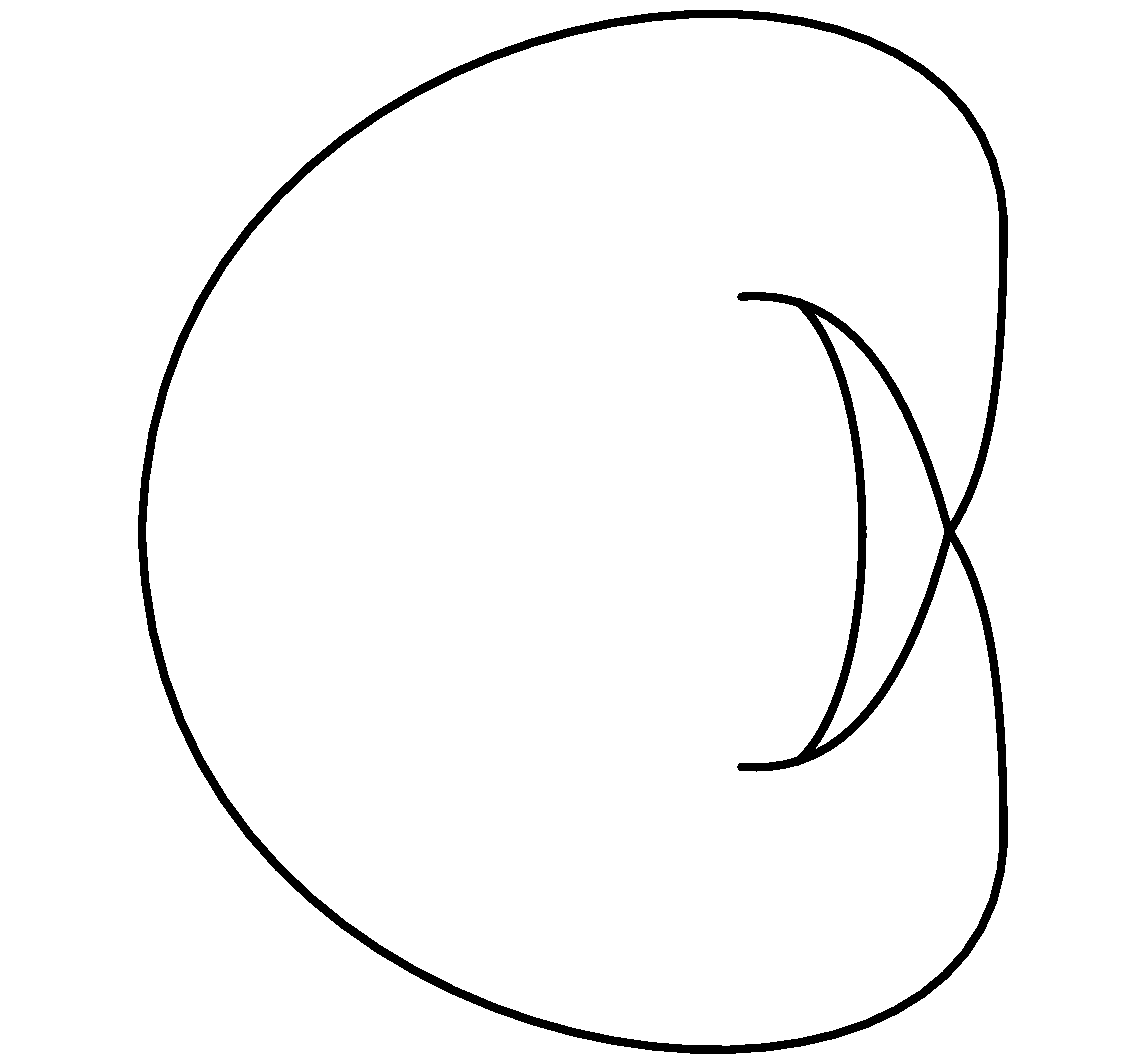
\includegraphics[width=.2\textwidth]{S2modS0.pdf}\hspace{7em}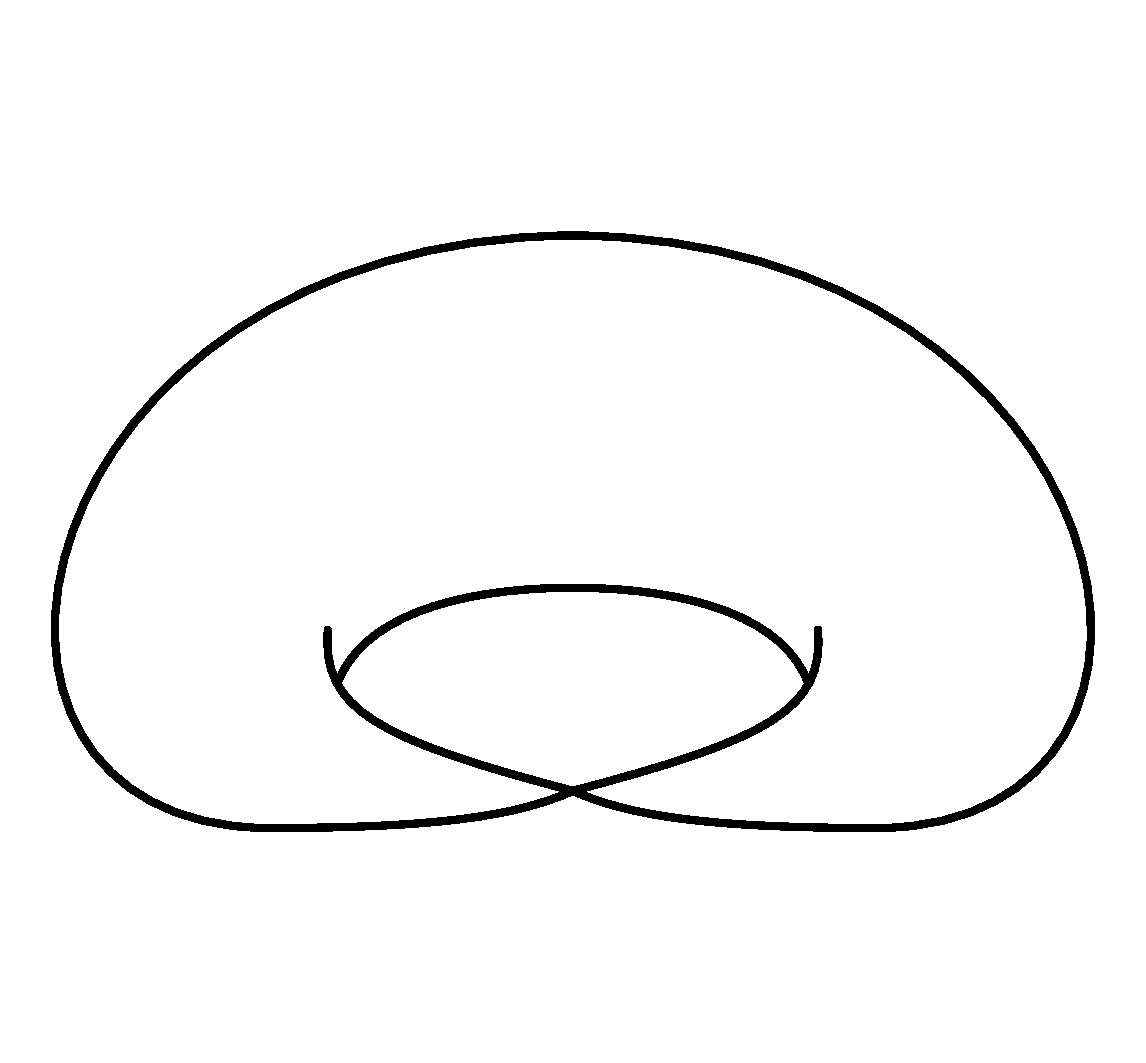
\includegraphics[width=.2\textwidth]{T2modS1.pdf}
					\end{center}
					Have LES of $(T^2,B)$,
					\begin{equation*}
						\begin{tikzcd}[column sep=small,row sep=tiny]
							\rhg[2]{B}\ar[d,equal]\ar[r]& \rhg[2]{T^2}\ar[r]& \rhg[2]{T^2,B}\ar[d,equal]\ar[r]& \rhg[1]{B}\ar[d,equal]\ar[r,"\iota_\ast"]& \rhg[1]{T^2}\ar[r]& \rhg[1]{T^2,B}\ar[d,equal]\ar[r]& \rhg[0]{B}\ar[d,equal]\\
							0 & & \Z & \Z & & \Z & 0
						\end{tikzcd}
					\end{equation*}
					\underline{Claim}: $\iota_\ast:\rhg[1]{B}\rightarrow \rhg[1]{T^2}$ is injective:\\
					$\pi:S^1\times S^1\rightarrow S^1, (x,y)\mapsto x$ then $\pi\circ\iota=\id_{S^1}$, $\pi_\ast\circ\iota_\ast=\id_{\rhg{S^1}}$ $\Rightarrow$ $\iota_\ast$ is injective.\\
					Split LES into SESs
					\begin{equation*}
						\begin{tikzcd}[row sep=tiny]
							0\ar[r]& \hg[2]{T^2}\ar[d,equal]\ar[r]& \hg[2]{T^2,B}\ar[d,equal]\ar[r]& \ker\iota_\ast\ar[d,equal]\ar[r]& 0\\
							& \Z & \Z & 0 &
						\end{tikzcd}
					\end{equation*}
					\begin{equation*}
						\begin{tikzcd}[row sep=tiny]
							0\ar[r]& \hg{B}\ar[d,equal]\ar[r]& \hg{T^2}\ar[r]& \hg{T^2,B}\ar[d,equal]\ar[r]& 0\\
							& \Z & & \Z & 
						\end{tikzcd}
					\end{equation*}
					We arrive at $\hg{T^2}=\begin{cases}
						\Z,&\ast=2\\\Z^2,& \ast=1\\0,&\text{else}
					\end{cases}$.
				\end{eg}

			
		\subsection{Subdivision, Excision and Collapsing}
			\subsubsection*{Subdivision}
				Suppose $\mathcal{U}=\{U_\alpha\}$ is an open cover of $X$.
				\vspace{1em}\\
				\noindent{\bfseries Notation:} If $\sigma:\Delta^k\rightarrow X$, write $\sigma\vartriangle \mathcal{U}$ if $\im\sigma\subset$ some $U_\alpha$.

				\begin{defi}
					$C_{k}^{\mathcal{U}}(X)=\langle \sigma|\sigma:\Delta^k\rightarrow X,\sigma\vartriangle \mathcal{U}\rangle$.	
				\end{defi}

				If $\im\sigma\subset U_\alpha$, then $\im\sigma\circ F_I\subset U_\alpha$, so $C_\ast^\mathcal{U}(X)$ is a subcomplex of $C_\ast(X)$. Let $i:C_\ast^\mathcal{U}(X)\rightarrow C_\ast(X)$ be the inclusion map.

				\begin{thm}(Subdivision)\label{thm--subdivision}
					Let $\mathcal{U}$ be an open cover of $X$. If $i:C_\ast^\mathcal{U}(X)\rightarrow \cx{X}$ is the inclusion, the induced map $i_\ast:H_\ast^\mathcal{U}(X)\rightarrow \hg{X}$ is an isomorphism.
				\end{thm}

				In particular, this ensures that the homology of $X$ is independent of the cover $\mathcal{U}$ we choose to compute $H_\ast^\mathcal{U}(X)$. This can be useful in cases where there are covers that admit to compute the homology easily compared to others.

				In order to prove this theorem we have to do some preparatory work first. We start by setting some notations about face maps. If $I\subset\{0,\dots,n\}$, we let $F_I:\Delta^{|I|}\rightarrow \Delta^n$be the corresponding face map. There is a chain map $\varphi_k:S_\ast(\Delta^k)\rightarrow \cx{\Delta^k}$ given by $\varphi_k(e_I)=F_I$. Let $f_I:S_\ast(\Delta^k)\rightarrow S_\ast(\Delta^n)$ be the chain map given by $f_I(e_I)=e_{I\circ J}:=e_{i_{j_0}\dots i_{j_l}}$, where $l=|J|$. Then we have $F_{I\circ J}=F_I\circ F_J$, which implies $\varphi_n\circ f_I=F_{I\#}\circ\varphi_k$. Finally, we define $\textbf{e}_n:=e_{01\dots n}\in S_n(\Delta^n)$ to be the top-dimensional face of $\Delta^n$.
				
				\begin{defi}
					If $X$ is a space, the cone on $X$ is $CX=(X\times[0,1])/(X\times\{0\})$.
				\end{defi}

				A map $f:X\rightarrow Y$ induces a map $Cf:CX\rightarrow CY$ given by $Cf(x,t)=(f(x),t)$. The cone $C\Delta^{n-1}$ can be identified with $\Delta^n$ by the map $\phi$ which sends $(x_0,\dots,x_{n-1},t)$ to $(1-t,tx_0,\dots,tx_{n-1})$. Thus, $\sigma:\Delta^{n-1}\rightarrow X$ induces a map $c\sigma:\Delta^n\rightarrow CX$ given by $c\sigma=C(\sigma\circ\phi^{-1})$. Hence, we have a map $c:\cx{X}\rightarrow \cx[\ast+1]{CX}$ given by $c(e_\sigma)=e_{c\sigma}$. If $i:X\rightarrow CX$ is the map given by $i(x)=(x,1)$, it follows easily from the definition that
				\begin{equation*}
					\mathrm{d}c(e_\sigma)=i_\#(e_\sigma)-c(\mathrm{d}e_\sigma).
				\end{equation*}
				
				Let $\pi:C\Delta^n\rightarrow \Delta^n, (\textbf{v},t)\mapsto t\textbf{v}+(1-t)\textbf{b}$ where $\textbf{b}=\frac{1}{n+1}(1,\dots,1)$ is the barycenter of $\Delta^n$, and define $\beta=\pi_\#\circ c:\cx{\Delta^n}\rightarrow \cx[\ast+1]{\Delta^n}$. Since $\pi\circ i=1_{\Delta^n}$, we have
				\begin{equation*}
					\mathrm{d}\beta(e_\sigma)=e_\sigma-\beta(\mathrm{d}e_\sigma).
				\end{equation*} 

				\begin{defi}(Barycentric subdivision)
					Define a chain map $B_n:\sx{\Delta^n}\rightarrow \cx{\Delta^n}$ inductively. First, $B_0:\sx[0]{\Delta^0}\rightarrow \cx[0]{\Delta^n}$ is uniquely defined by the requirement that $B_0(e_0)=e_p$, where $p$ is the unique point of $\Delta_0$. In general, if $I$ is a proper subset of $\{0,\dots,n\}$, we define
					\begin{equation*}
						B_n(e_I)=F_{I\#}(B_{|I|}(e_{|I|})).
					\end{equation*}
					Finally, we define
					\begin{equation*}
						B_n(\textbf{e}_n)=\beta(B_n(\mathrm{d}\textbf{e}_n))\in\cx[n]{\Delta^n}.
					\end{equation*}
				\end{defi}

				Observe that all the singular simplices appearing in the image of $B_n$ are given by affine linear maps.

				\begin{lemma}
					$B_n$ is a chain map.
				\end{lemma}
				\begin{proof}
					This is proved by induction on $n$. The case $n=0$ is trivial. Given that $B_k$ is a chain map for $k<n$, it follows from the definition that $B_n$ is a chain map when restricted to $\sx{\Delta^n}$ where $\ast<n$. Thus, the only thing to check is that $B_n(\mathrm{d}\textbf{e}_n)=\mathrm{d}B_n(\textbf{e}_n)$. We compute
					\begin{align*}
						\mathrm{d}B_n(\textbf{e}_n)=&\mathrm{d}\beta(B_n(\mathrm{d}\textbf{e}_n))\\
						=&B_n(\mathrm{d}\textbf{e}_n)-\beta(\mathrm{d}B_n(\mathrm{d}\textbf{e}_n))\\
						=&B_n(\mathrm{d}\textbf{e}_n)-\beta(B_n(\mathrm{d}^2\textbf{e}_n))\\
						=&B_n(\mathrm{d}\textbf{e}_n).
					\end{align*}
					We have used the fact thet statement holds in gradings $<n$ in passing from the second to the third line.
				\end{proof}

				Next, we want to define a chain homotopy $T_n:\sx{\Delta_n}\rightarrow \cx[\ast+1]{\Delta^n}$. As with the chain map $B_n$, we define $T_n$ inductively. First, let $T_0$ be the trivial map. Next, if $I$ is a proper subset of $0,\dots,n$, define
				\begin{equation*}
					T_n(e_I)=F_{I\#}(T_{|I|}(\textbf{e}_{|I|})).
				\end{equation*}
				Finally, we define 
				\begin{equation*}
					T_n(\textbf{e}_n)=\beta(B_n(\textbf{e}_n)-\varphi_n(e_n)-T_n(\mathrm{d}\textbf{e}_n)).
				\end{equation*}

				\begin{lemma}
					$\mathrm{d}T_n+T_n\mathrm{d}=B_n-\varphi_n$.
				\end{lemma}
				\begin{proof}
					This is proved by induction on $n$. The case $n=0$ is easily verified, since $T_0=0$ and $B_0=\phi_0$. Suppose the result holds for all $k<n$. As in the case of $B_n$, we need only verify the identity when both sides are applied to $\textbf{e}_n$; the other cases follow from the induction hypothesis. For $\textbf{e}_n$, we compute
					\begin{align*}
						\mathrm{d}T_n(\textbf{e}_n)=&\mathrm{d}\beta(B_n(\textbf{e}_n)-\varphi_n(\textbf{e}_n)-T_n(\mathrm{d}\textbf{e}_n))\\
						=&B_n(\textbf{e}_n)-\varphi_n(\textbf{e}_n)-T_n(\mathrm{d}\textbf{e}_n)-\beta(B_n(\mathrm{d}\textbf{e}_n)-\varphi_n(\mathrm{d}\textbf{e}_n)-\mathrm{d}T_n(\mathrm{d}\textbf{e}_n))\\
						=&B_n(\textbf{e}_n)-\varphi_n(\textbf{e}_n)-T_n(\mathrm{d}\textbf{e}_n)-\beta(T_n(\mathrm{d}^2\textbf{e}_n))\\
						=&B_n(\textbf{e}_n)-\varphi_n(\textbf{e}_n)-T_n(\mathrm{d}\textbf{e}_n)
					\end{align*}
					where we have used the fact that the identity holds for $e_I$ with $|I|<n$ in going from the second to the third line. So $\mathrm{d}T_n(\textbf{e}_n)+T_n(\mathrm{d}\textbf{e}_n)=B_n(\textbf{e}_n)-\varphi_n(\textbf{e}_n)$ as desired.
				\end{proof}

				\begin{lemma}\label{lem--naturality}
					If $F_I:\Delta^k\rightarrow \Delta^n$ is a face map, then $B_n\circ f_I=F_{I\#}\circ B_k$ and $T_n\circ f_I=F_{I\#}\circ T_k$.
				\end{lemma}
				\begin{proof}
					We have
					\begin{equation*}
						B_n(f_I(e_J))=B_n(e_{I\circ J})=(F_{I\circ J})_\#(B_{|J|}(\textbf{e})_{|J|})=F_{I\#}(F_{J\#}(B_{|J|}(\textbf{e}_{|J|})))=F_{I\#}(B_k(e_J)).
					\end{equation*}
					The proof of the second statement is identical, but with $B$'s replaced by $T$'s.
				\end{proof}
				
				If $X$ is a space, define $B:\cx{X}\rightarrow \cx{X}$ by $B(e_\sigma)=\sigma_\#(B_n(\textbf{e}_n))$ for $\sigma:\Delta^n\rightarrow X$. It is clear from the definition that if $g:X\rightarrow Y$, then $B(g_\#(e_\sigma))=g_\#(B_n(e_\sigma))$.

				\begin{lemma}
					$B$ is a chain map.
				\end{lemma}
				\begin{proof}
					We compute
					\begin{align*}
						B(\mathrm{d}e_\sigma)=&\sum(-1)^jB(e_{\sigma\circ F_{\overset{\curlywedge}{j}}})\\
						=&\sum(-1)^j\sigma_{\#}(F_{\overset{\curlywedge}{j}\#}(B_{n-1}(\textbf{e}_{n-1})))\\
						=&\sum(-1)^j\sigma_{\#}(B_n(f_{\overset{\curlywedge}{j}}(\textbf{e}_{n-1})))\qquad\text{(by \autoref{lem--naturality})}\\
						=&\sigma_{\#}(B_n(\mathrm{d}\textbf{e}_n))\\
						=&\sigma_{\#}(\mathrm{d}B_n(\textbf{e}_n))\qquad\text{($B_n$ is a chain map)}\\
						=&\mathrm{d}B(e_\sigma).
					\end{align*}
				\end{proof}

				\begin{lemma}
					$B$ is chain homotopic to $1_{\cx{X}}$.
				\end{lemma}
				\begin{proof}
					Let us define $T:\cx{X}\rightarrow\cx[\ast+1]{X}$ by $T(e_\sigma)=\sigma_{\#}(T_n(\textbf{e}_n))$. As in the previous lemma, we compute
					\begin{align*}
						T(\mathrm{d}e_\sigma)=&\sum(-1)^jT(e_{\sigma\circ F_{\overset{\curlywedge}{j}}})\\
						=&\sum(-1)^j\sigma_{\#}(F_{\rmv{j}\#}(T_{n-1}(\textbf{e}_{n-1})))\\
						=&\sum(-1)^j\sigma_{\#}(T_n(f_{\rmv{j}}(\textbf{e}_{n-1})))\qquad\text{(by \autoref{lem--naturality})}\\
						=&\sigma_{\#}(T_n(\mathrm{d}\textbf{e}_n)).
					\end{align*}
					Somewhat more easily, we have $\mathrm{d}T(e_\sigma)=\sigma_{\#}(\mathrm{d}T_n(e_n))$, so
					\begin{equation*}
						\mathrm{d}T(e_\sigma)+T\mathrm{d}(e_\sigma)=\sigma_{\#}(\mathrm{d}T_n(e_n)+T_n(\mathrm{d}e_n))=\sigma_{\#}(B_n(e_n)-\varphi_n(e_n))=B(e_\sigma)-e_\sigma.
					\end{equation*}
				\end{proof}

				Now let $\textbf{F}_n=\phi_n(\textbf{e}_n)\in\cx[n]{\Delta^n}$ be the singular simplex corresponding to the map $1_{\Delta^n}$. If $\sigma:\Delta^n\rightarrow X$, then $e_\sigma=\sigma_{\#}(\textbf{F}_n)$, so $B_r(e_\sigma)=\sigma_{\#}(B_r(\textbf{F}_n))$. The simplices appearing in $B_r(\textbf{F}_n)$ are all affine linear simplices obtained by iteratively applying barycentric subdivision to $\Delta^n$.

				\begin{lemma}
					If $\Delta$ is an affine linear simplex of dimension $n$, and $\Delta^{\prime}$ is a simplex obtained by applying barycentric subdivision to $\Delta$, then $\diam(\Delta^{\prime})\le \frac{n}{n+1}\diam(\Delta)$.
				\end{lemma}
				\begin{proof}
					Let $\textbf{v}_0,\dots,\textbf{v}_n$ be the vertices of $\Delta$, so $d=\diam(\Delta)=\max\norm{\textbf{v}_i-\textbf{v}_j}$. We induct on $n$. Suppose $\textbf{v},\textbf{v}^{\prime}$ are two vertices of $\Delta^{\prime}$. If $\textbf{v},\textbf{v}^{\prime}$ lie in a $k$-dimensional proper face $\Delta_I$ of $\Delta$, they are vertices of a simplex appearing in the barycentric subdivision of $\Delta_I$. By induction we have $\norm{\textbf{v}-\textbf{v}^{\prime}}\le\frac{k}{k+1}\diam(\Delta_I)\le\frac{n}{n+1}d$. So it suffices to consider the case where $\textbf{v}=\frac{n}{n+1}(\textbf{v}_0+\dots+\textbf{v}_n)$ is the barycenter. Without loss of generality, we may assume the other vertex is of the form $\frac{1}{k+1}(\textbf{v}_0+\dots+\textbf{v}_n)$ for some $k$. Then,
					\begin{equation*}
						\textbf{v}^{\prime}-\textbf{v}=\frac{1}{(n+1)(k+1)}[(n-k)\textbf{v}_0+\dots+(n-k)\textbf{v}_k-(k+1)\textbf{v}_{k+1}-\dots-(k+1)\textbf{v}_{n}].
					\end{equation*} 
					The sum in the parentheses on the RHS can be rearranged into a sum of $(n-k)(k+1)$ terms of the form $\textbf{v}_i-\textbf{v}_j$, so 
					\begin{equation*}
						\norm{\textbf{v}^{\prime}-\textbf{v}}\le\frac{n-k}{n+1}\max\norm{\textbf{v}_i-\textbf{v}_j}=\frac{n-k}{n+1}\,d\le\frac{n}{n+1}d.
					\end{equation*}
				\end{proof}

				\begin{cor}\label{cor--diameter}
					If we normalise $\Delta^n$ to have diameter 1, then every simplez appearing in $B_r(\textbf{F}_n)$ has diameter less or equal to $\left(\frac{n}{n+1}\right)^r$.
				\end{cor}

				We will use the following standard fact about metric spaces:

				\begin{lemma}\label{lem--metricspace}
					If $\{U_i\}$ is an open cover of a compact metric space $X$, then there is some $\epsilon>0$ so that any $A\subset X$ with diameter $<\epsilon$ is contained in some $U_i$.
				\end{lemma}
				
				\begin{prop}\label{prop--11}
					Let $\mathcal{U}$ be an open cover of $X$. If $c\in\cx{X}$, there is some $r>0$ so that $B_r(c)\in C_\ast^{\mathcal{U}}(X)$.
				\end{prop}
				\begin{proof}
					Since any $c\in\cx{X}$ is a finite linear combination of singular simplices, it suffices to prove the claim in the case where $c=e_\sigma$. Let $V_i=\sigma^{-1}(U_i)$. Then the $V_i$ are an open cover of $\Delta^n$, so we can apply \autoref{lem--metricspace} to find an $\epsilon>0$ such that any $A\subset X$ with diameter $<\epsilon$ is contained in some $V_i$. By \autoref{cor--diameter}, we can choose $r$ so that the diameter of any simplex in $B_r(\textbf{F}_n)$ is $<\epsilon$. Thus, any simplex appearing in $B_r(\textbf{F}_n)$ is contained in some $V_i$. Since $B_r(e_\sigma)=\sigma_{\#}(B_r(\textbf{F}_n))$, every singular simplex appearing in $B_r(e_\sigma)$ is contained in some $U_i$.
				\end{proof}

				\begin{proof}(of \autoref{thm--subdivision})
					We first show the map $i_\ast:H_\ast^\mathcal{U}(X)\rightarrow\hg{X}$ is surjective. Given $[c]\in\hg{X}$, we apply \autoref{prop--11} to see that $B_r(c)\in C_\ast^\mathcal{U}(X)$ for some $r$. Now $B_r\sim 1_{\cx{X}}$, so $[c]=[B_r(c)]$. It follows that $i_\ast$ is surjective. Next, we show that $i_\ast$ is injective. If $[c]\in H_\ast^\mathcal{U}$ and $c=\mathrm{d}y$ for some $y\in\cx{X}$, then we can find $r$ so that $B_r(y)\in C_\ast^\mathcal{U}(X)$. Since $B$ is a chain map, $B_r(c)=B_r(\mathrm{d}y)=\mathrm{d}B_r(y)$, so $[c]=[B_r(c)]=0$ in $H_\ast^\mathcal{U}(X)$.
				\end{proof}

				There is a very useful application of the subdivision theorem which we write down at once.

				\begin{prop}(Mayer-Vietoris sequence)
					Suppose $U_1,U_2\subset X$ are open and $U_1\cup U_2=X$, i.e. $\mathcal{U}=\{U_1,U_2\}$ is an open cover of $X$,
					\begin{equation*}
						\begin{tikzcd}
							& U_1\ar[rd,"j_1"] & \\
							U_1\cap U_2\ar[ru,"l_1"]\ar[rd,"l_2"]& & X\\
							& U_2\ar[ru,"j_2"] &
						\end{tikzcd}.
					\end{equation*}
					There is a LES
					\begin{equation*}
						\begin{tikzcd}[column sep=scriptsize]
							\dots\ar[r]& \hg{U_1\cap U_2}\ar[r,"l_{1\ast}\oplus l_{2\ast}"]& \hg{U_1}\oplus\hg{U_2}\ar[r,"j_{1\ast}-j_{2\ast}"]& \hg{X}\ar[r,"\partial"]& \hg[\ast-1]{U_1\cap U_2}\ar[r]& \dots
						\end{tikzcd}
					\end{equation*}
				\end{prop}
				\begin{proof}
					There is a SES
					\begin{equation*}
						\begin{tikzcd}
							0\ar[r]& \cx{U_1\cap U_2}\ar[r,"l_{1\#}\oplus l_{2\#}"]& \cx{U_1}\oplus\cx{U_2}\ar[r,"j_{1\#}-j_{2\#}"]& C_\ast^\mathcal{U}(X)\ar[r]& 0.
						\end{tikzcd}
					\end{equation*}
					Take LES of homology and use $H_\ast^\mathcal{U}(X)\simeq\hg{X}$.
				\end{proof}

				We obtain a similar sequenece for the reduced homology $\rhg{X}$.

				\begin{eg}
					Let $X=S^n$ and choose $U_1=S^n\backslash\{p\},U_2=S^n\backslash\{q\}$. Then $U_1\cap U_2\simeq\inte D^n\backslash\{0\}\simeq S^{n-1}$. Mayer-Vietoris yields the sequence
					\begin{equation}
						\begin{tikzcd}[row sep=tiny]
							\rhg{U_1}\oplus\rhg{U_2}\ar[d,equal]\ar[r]& \rhg{S^n}\ar[r]& \rhg[\ast-1]{U_1\cap U_2}\ar[d,equal]\ar[r]& \rhg[\ast-1]{U_1}\oplus\rhg[\ast-1]{U_2}\ar[d,equal]\\
							0 & & \rhg[\ast-1]{S^{n-1}} & 0
						\end{tikzcd}
					\end{equation}
					and thus $\rhg{S^n}\simeq\rhg[\ast-1]{S^{n-1}}$.
				\end{eg}

			\subsubsection*{Excision}
				Suppose $A\subset X$, $\mathcal{U}$ is an open cover of $X$. Let $\mathcal{U}_A=\{U_\alpha\cap A\}$ an open cover of $A$. Then $C_\ast^{\mathcal{U}_A}(A)$ is a subcomplex of $C_\ast^\mathcal{U}(X)$. Define $C_\ast^\mathcal{U}(X,A):=\frac{C_\ast^\mathcal{U}(X)}{C_\ast^{\mathcal{U}_A}(A)}$.

				\begin{lemma}
					(Five lemma) Suppose we have a commuting diagram
					\begin{equation*}
						\begin{tikzcd}
							A_1\ar[d,"f_1"]\ar[r]& A_2\ar[d,"f_2"]\ar[r]& A_3\ar[d,"f_3"]\ar[r]& A_4\ar[d,"f_4"]\ar[r]& A_5\ar[d,"f_5"]\\
							B_1\arrow[ur, phantom, "\scalebox{1.5}{$\circlearrowleft$}" description]\ar[r]& B_2\arrow[ur, phantom, "\scalebox{1.5}{$\circlearrowleft$}" description]\ar[r]& B_3\arrow[ur, phantom, "\scalebox{1.5}{$\circlearrowleft$}" description]\ar[r]& B_4\arrow[ur, phantom, "\scalebox{1.5}{$\circlearrowleft$}" description]\ar[r]& B_5
						\end{tikzcd}
					\end{equation*}
					with exact rows and $f_1,f_2,f_4,f_5$ all isomorphisms. Then also $f_3$ is an isomorphism.
				\end{lemma}
				\begin{proof}
					We show (i) $f_2,f_4$ monomorphisms, $f_1$ epimorphism $\Longrightarrow$ $f_3$ monomorphism and (ii) $f_2,f_4$ epimorphism, $f_5$ monomorphism $\Longrightarrow$ $f_3$ epimorphism.
					\begin{enumerate}
						\item[(i):] \begin{equation*}
							\begin{tikzcd}
								\exists x_1\ar[d,mapsto]\ar[r,mapsto]& x_2^{\prime},\exists x_2\ar[d,mapsto,xshift=-2.5ex,end anchor=north east]\ar[d,mapsto,xshift=2.5ex,end anchor=north west]\ar[r,mapsto]& x_3\in\ker f_3\ar[d,mapsto]\ar[r]& x_4=0\ar[d,mapsto]\\
								\exists y_1\ar[r,mapsto]& y_2\ar[r,mapsto]& 0\ar[r,mapsto]& 0
							\end{tikzcd}
						\end{equation*}
						But $f_2$ monomorphism $\Rightarrow$ $x_2^{\prime}=x_2$ $\Rightarrow$ $x_3=0$ (exact at $A_2$).
						\item[(ii):] \begin{equation*}
							\begin{tikzcd}
								\exists x_2\ar[d,mapsto]\ar[r,mapsto]& x_3^{\prime},\exists x_3\ar[dd,mapsto,xshift=-2ex,controls={+(-.1,-0.4) and +(-.4,0.8)}]\ar[d,mapsto,xshift=2.5ex,end anchor=north west]\ar[r,mapsto]& \exists x_4\ar[d,mapsto]\ar[r,mapsto]& x_5=0\ar[d,mapsto,xshift=-2.3ex]\\
								\exists y_2\ar[rd,mapsto] & y_3^{\prime},y_3\ar[r,mapsto,xshift=-4ex,controls={+(.5,-.4) and +(-.3,-.7)},end anchor=south east]\ar[r,mapsto]& y_4\ar[r,mapsto]& y_5=0\\
								& y_3^{\prime\prime}=y_3-y_3^{\prime}\ar[r,mapsto]& 0 &
							\end{tikzcd}
						\end{equation*}
						Thus, $x_3^{\prime}+x_3\mapsto y_3^{\prime\prime}+y_3^{\prime}=y_3$, so $f_3$ epimorphism.
					\end{enumerate}
				\end{proof}

				\begin{cor}\label{cor--excision}
					$H_\ast^\mathcal{U}(X,A)\simeq\hg{X,A}$.
				\end{cor}
				\begin{proof}
					There is a map of SESs
					\begin{equation*}
						\begin{tikzcd}
							0\ar[r]& C_\ast^{\mathcal{U}_A}(A)\ar[d]\ar[r]& C_\ast^\mathcal{U}(X)\ar[d]\ar[r]& C_\ast^\mathcal{U}(X,A)\ar[d]\ar[r]& 0\\
							0\ar[r]& \cx{A}\ar[r]& \cx{X}\ar[r]& \cx{X,A}\ar[r]& 0
						\end{tikzcd}
					\end{equation*}
					so we get a map of LESs of homology
					\begin{equation*}
						\begin{tikzcd}
							\shg{_A}{A}\ar[d]\ar[r]& \shg{}{X}\ar[d]\ar[r]& \shg{}{X,A}\ar[d]\ar[r]& \shg[\ast-1]{_A}{A}\ar[d]\ar[r]& \shg[\ast-1]{}{X}\ar[d]\\
							\hg{A}\ar[r]& \hg{X}\ar[r]& \hg{X,A}\ar[r]& \hg[\ast-1]{A}\ar[r]& \hg[\ast-1]{X}
						\end{tikzcd}
					\end{equation*}
					Arrows 1,2,4,5 are isomorphisms by subdivision, so 3 is isomorphism by the Five lemma.
				\end{proof}

				\begin{thm}(Excision)
					Suppose $B\subset A\subset X$, $j:(X- B,A- B)\rightarrow (X,A)$ inclusion. If $\bar{B}\subset\inte A$, then $j_\ast:\hg{X- B,A- B}\rightarrow \hg{X,A}$ is an isomorphism.
				\end{thm}
				\begin{proof}
					$\bar{B}\subset\inte A$, so $\mathcal{U}=\{X-\bar{B}, \inte A\}$ is an open cover of $X$. Then
					\begin{align*}
						\scx{}{X}=&\langle \sigma|\sigma\vartriangle\mathcal{U},\im\sigma\cap\bar{B}=\emptyset\rangle\oplus\langle \sigma|\sigma\vartriangle U,\im\sigma\cap B\neq\emptyset\rangle\\
						=&\scx{^{\prime}}{X- B}\oplus\langle \sigma|\im\sigma\subset\inte A\rangle,
					\end{align*}
					where $\mathcal{U}^{\prime}=U_{X- B}$.
					Similarly, $\scx{_A}{A}=\scx{_A^{\prime}}{A- B}\oplus\langle \sigma|\im\sigma\subset\inte A\rangle$, so
					\begin{equation*}
						\frac{\scx{}{X}}{\scx{_A}{A}}\simeq\frac{\scx{^{\prime}}{X- B}}{\scx{_A^{\prime}}{A- B}},
					\end{equation*}
					i.e. 
					\begin{equation*}
						\begin{tikzcd}
							j_\#^\mathcal{U}:\scx{^{\prime}}{X- B,A- B}\ar[d,"\iota^{\prime}"]\ar[r]& \scx{}{X,A}\ar[d,"\iota"]\\
							\cx{X- B,A- B}\ar[r,"j_\#"]& \cx{X,A}
						\end{tikzcd}
					\end{equation*}
					is an isomorphism. By \autoref{cor--excision}, $\iota_\ast^{\prime}$ and $\iota_\ast$ are isomorphisms and $j_\ast^\mathcal{U}$ is an isomorphism because $j_\#^\mathcal{U}$ is. Hence, $j_\ast$ is an isomorphism.
				\end{proof}

				\begin{eg}
					\begin{enumerate}
						\item $\hg{\R^n,\R^n\backslash\{p\}}=\begin{cases}
							\Z,&\ast=n\\
							0,&\ast\neq n
						\end{cases}$.
						\begin{proof}
							$\R^n\backslash\{p\}\simeq\R^n\backslash\{0\}\sim S^{n-1}$, LES
							\begin{equation*}
								\begin{tikzcd}[row sep=tiny]
									\rhg{\R^n}\ar[d,equal]\ar[r]& \hg{\R^n,\R^n\backslash\{p\}}\ar[r,"\partial"]& \rhg[\ast-1]{\R^n\backslash\{p\}}\ar[r]& \rhg[\ast-1]{\R^n}\ar[d,equal]\\
									0 & & & 0
								\end{tikzcd}
							\end{equation*}
							so $\partial:\hg{\R^n,\R^n\backslash\{p\}}\overset{\simeq}{\longrightarrow }\hg[\ast-1]{S^{n-1}}$. NB: $\rhg{\R^n/(\R^n\backslash\{p\})}$ does not depend in $n$.
						\end{proof}
						\item If $U\subset\R^n$ is open, then $\hg{U,U\backslash\{p\}}=\begin{cases}
							\Z,&\ast=n\\0,&\ast\neq n
						\end{cases}$.
						\begin{proof}
							$C=\R^n\backslash U$ is closed in $\R^n$, so $\bar{C}\subset\R^n\backslash\{p\}$. By excision,
							\begin{equation*}
								\hg{\R^n,\R^n\backslash\{p\}}\simeq\hg{\R^n\backslash C,\R^n\backslash \{p\}\backslash C}=\hg{U,U\backslash\{p\}}.
							\end{equation*}
						\end{proof}
					\end{enumerate}
				\end{eg}

				\begin{cor}
					If $U\subset\R^n, V\subset\R^m$ are open and $U\simeq V$ (homeomorphic), then $n=m$.
				\end{cor}
				\begin{proof}
					If $f:U\overset{\simeq}{\longrightarrow}V$, then $(U,U\backslash\{p\})\overset{\simeq}{\mapsto}(V,V\backslash \{f(p)\})$, so
					\begin{equation*}
						\hg{U,U\backslash\{p\}}\simeq\hg{V,V\backslash\{f(p)\}}.
					\end{equation*}
				\end{proof}

			\subsubsection*{Deformation Retractions}
				Suppose $A\subset U$, let $\iota:A\rightarrow U$ be the inclusion. If $\pi:U\rightarrow A$, have maps of pairs
				\begin{equation*}
					\begin{tikzcd}
						(U,A)\ar[r,"\tilde{\pi}"]& (A,A)\ar[r,"\tilde{\iota}"]& (U,A)
					\end{tikzcd}
				\end{equation*}

				\begin{defi}
					$\pi:U\rightarrow A$ is a deformation retraction if $\tilde{\iota}\circ\tilde{\pi}\sim\id_{(U,A)}$ as maps of pairs.
				\end{defi}

				\begin{lemma}\label{lem--1}
					If $\pi:U\rightarrow A$ is a deformation retract so is $\pi^{\prime}:U/A\rightarrow A/A$.
				\end{lemma}

				\begin{lemma}
					(LES of triple) Suppose $B\subset A\subset X$. Then there is a LES
					\begin{equation*}
						\begin{tikzcd}
							\dots\ar[r]& \hg{A,B}\ar[r,"j_\ast"]& \hg{X,B}\ar[r,"i_\ast"]& \hg{X,A}\ar[r,"\partial"]& \hg[\ast-1]{A,B}\ar[r]& \dots 
						\end{tikzcd}
					\end{equation*}
					with $j_\ast,i_\ast$ induced by inclusions of pairs.	
				\end{lemma}
				\begin{proof}
					There is a SES
					\begin{equation*}
						\begin{tikzcd}
							0\ar[r]& \frac{\cx{A}}{\cx{B}}\ar[r,"i_\#"]& \frac{\cx{X}}{\cx{B}}\ar[r,"j_\#"]& \frac{\cx{X}}{\cx{A}}\ar[r]& 0.
						\end{tikzcd}
					\end{equation*}
				\end{proof}

				\begin{lemma}\label{lem--3}
					Suppose $A\subset U\subset X$ and $A$ is a deformation retract of $U$. Then the map $\iota_\ast:\hg{X,A}\rightarrow\hg{X,U}$ is an isomorphism.
				\end{lemma}
				\begin{proof}
					$\iota:A\rightarrow U$ is a homotopy equivalence ($A$ deformation retract), so $\iota_\ast:\hg{A}\overset{\simeq}{\longrightarrow}\hg{U}$. The LES of $(U,A)$ gives
					\begin{equation*}
						\begin{tikzcd}[row sep=tiny]
							0\ar[r]& (\coker\iota_\ast)_n\ar[d,equal]\ar[r]& \hg{U,A}\ar[r]& (\ker\iota_\ast)_{n-1}\ar[d,equal]\ar[r]& 0\\
							& 0 & & 0 &
						\end{tikzcd}
					\end{equation*}
					so $\hg{U,A}=0$. The LES of the triple $(X,U,A)$ gives 
					\begin{equation*}
						\begin{tikzcd}[row sep=tiny]
							\hg{U,A}\ar[d,equal]\ar[r]& \hg{X,A}\ar[r,"\iota_\ast"]& \hg{X,U}\ar[r]& \hg[\ast-1]{U,A}\ar[d,equal]\\
							0 & & & 0
						\end{tikzcd}
					\end{equation*}
					so $\iota_\ast$ is an isomorphism.
				\end{proof}

				We are now in a position to prove \autoref{thm--subdivision}, whose proof we had postponed in order to build some more machinery first.

				\begin{proof}(of \autoref{thm--subdivision})
					\begin{equation*}
						\begin{tikzcd}
							\hg{X,A}\ar[d,"\pi_\ast"]\ar[r,"\iota_\ast"]& \hg{X,U}\ar[d,"\pi_{2\ast}"]& \hg{X- A,U- A}\ar[d,"\pi_{3\ast}"]\ar[l,"j_\ast"']\\
							\hg{X/A,A/A}\arrow[ur, phantom, "\scalebox{1.5}{$\circlearrowleft$}" description]\ar[r,"\iota_\ast^{\prime}"]& \hg{X/A,U/A}\arrow[ur, phantom, "\scalebox{1.5}{$\circlearrowleft$}" description]& \hg{X/A-A/A,U/A-A/A}\ar[l,"j_\ast^{\prime}"']
						\end{tikzcd}
					\end{equation*}
					Now $\pi_{3}:(X-A,U-A)\rightarrow (X/A-A/A,U/A-A/A)$ is a homeomorphism, so $\pi_{3\ast}$ is an isomorphism. $A$ is closed and $U$ is open, so $\bar{A}\subset\inte U$. By excision, $j_\ast,j_\ast^{\prime}$ are isomorphisms, hence, so is $\pi_{2\ast}$. By \autoref{lem--1} and \ref{lem--3}, $\iota_\ast$ and $\iota_\ast^\prime$ are isomorphisms. Therefore, finally, $\pi_\ast$ is an isomorphism, as advertised.
				\end{proof}


		
		\subsection{Maps $S^n\rightarrow S^n$}
			Fix generators for $\rhg[n]{S^n}\simeq\Z$ (e.g. $S^0=\{-1,1\},[S^0]=\sigma_1-\sigma_{-1}$ generates $\rhg[0]{S^0}$). We have isomorphisms
			\begin{equation*}
				\begin{tikzcd}
					\overset{[S^n]}{\rhg[n]{S^n}}& \overset{[D^n,S^{n-1}]}{\hg[n]{D^n,S^{n-1}}}\ar[d,"\partial"]\ar[l,"p_\ast"']\ar[r,"f_\ast"]& \overset{[I^n,\partial I^n]}{\hg[n]{I^n,\partial I^n}}\simeq\Z\\
					& \underset{[S^{n-1}]}{\rhg[n-1]{S^{n-1}}} &
				\end{tikzcd}.
			\end{equation*}
			If $f:S^n\rightarrow S^n$, then the induced map $f_\ast:\hg[n]{S^n}\rightarrow \hg[n]{S^n}$ is a homomorphism from $\Z$ to itself and hence we must have $f_\ast[S^n]=k[S^n]$ with $k\in\Z$.

			\begin{defi}
				(Degree of a map) Let $f:S^n\rightarrow S^n$ as above, then we set $\deg f:=k$ the degree of $f$.
			\end{defi}

			\noindent{\bfseries Properties:}\begin{enumerate}
				\item $\deg(f\circ g)=\deg f\cdot\deg g$, for $(f\circ g)_\ast=f_\ast\circ g_\ast$
				\item $f\sim g\Longrightarrow \deg f=\deg g$, for $f_\ast=g_\ast$
				\item $\deg\id_{S^n}=1$, for $(\id_{S^n})_\ast=\id$
				\item If $f:S^n\rightarrow S^n$ is not surjctive, then $\deg f=0$.
					\begin{proof}
						If $f$ not surjective, have $y_0\in S^n-f(S^n)$ such that we have
						\begin{equation*}
							\begin{tikzcd}[column sep=scriptsize]
								f:S^n\ar[rd]\ar[rr]& & S^n\\
								& S^n-\{y_0\}\ar[ru,hookrightarrow,"\iota"] &
							\end{tikzcd}.
						\end{equation*}
						But $S^n-\{y_0\}\sim D^n$, so $\hg{S^n-\{y_0\}}=0$. Therefore, $\iota_\ast=0$ and thus $f_\ast=0$. 
					\end{proof}
				
				\item If $f:S^n\overset{\simeq}{\longrightarrow} S^n$ is a homeomorphism, then $\deg f=\pm 1$.
					\begin{proof}
						$1=\deg\id_{S^n}=\deg(f\circ f^{-1})=\deg f\cdot\deg f^{-1}$ $\Longrightarrow$ $\deg f$ is a unit in $\Z$.
					\end{proof}
			\end{enumerate}

			\begin{prop}
				If $p:S^n\rightarrow S^n$ is a reflection in a hyperplane, then $\deg p=-1$.
			\end{prop}
			\begin{proof}
				The reflection fixe the points in a subsphere $S^{n-1}$ and exchanges the two hemispheres. Give $S^n$ a $\Delta$-complex structure with the two $n$-simplices $\Delta_1^n,\Delta_2^n$ the two hemispheres. Then $\Delta_1^n-\Delta_2^n$ generates $\hg[n]{S^n}$.
			\end{proof}

			\begin{cor}
				If $A:S^n\rightarrow S^n, v\mapsto -v$ is the antipodal map, then $\deg A=(-1)^{n+1}$.
			\end{cor}
			\begin{proof}
				$A=p_1\circ p_2\circ \dots\circ p_{n+1}$, where $p_i(v)=(v_1,\dots,-v_i,\dots,v_{n+1})$ is a reflection.
			\end{proof}

			\begin{cor}
				If $n$ is even, $A\not\sim\id_{S^n}$.
			\end{cor}

			\subsubsection*{Hurewicz Homomorphism}
				\begin{defi}
					The Hurewicz homomorphism is $\psi:\pi_n(X,p)\rightarrow \hg[n]{X}$ with $\psi([\tilde{\alpha}])=\tilde{\alpha}_\ast[S^n]$, $\psi([\alpha])=\alpha_\ast[I^n,\partial I^n]$, where
					\begin{equation*}
						\begin{tikzcd}
							\tilde{\alpha}:(S^n,\ast)\ar[r]& (X,p)\\
							(I^n,\partial I^n)\ar[u,"\pi"]\ar[ur,"\alpha"]&
						\end{tikzcd}.
					\end{equation*}
					$\psi$ is well defined: $\alpha\sim\beta$, then $\alpha_\ast=\beta_\ast$.
				\end{defi}
			
				\begin{prop}\label{prop--hurewicz}
					We have $\psi([\alpha+\beta])=\psi([\alpha])+\psi([\beta])$.
				\end{prop}
				
				The proof of \autoref{prop--hurewicz} is postponed at this point and will be provided after some more work. 
				According to the proposition above, $\psi:\pi_n(S^n,\ast)\rightarrow\hg[n]{[S^n]}\simeq\Z, f\mapsto\deg f$ is a homomorphism. Moreover, $\psi(\id_{S^n})=1$ and therefore $\psi$ is surjective. Define $R:I^n\rightarrow I^n, (x,\vec{x})\rightarrow(1-x,\vec{x})$.

				\begin{lemma}
					It is $[\alpha]+[\alpha\circ R]=0$ in $\pi_n(S^n)$, i.e. $[\alpha\circ R]=-[\alpha]$.
				\end{lemma}

				\begin{cor}
					$R_\ast[I^n,\partial I^n]=-[I^n,\partial I^n]$.
				\end{cor}
				\begin{proof}
					$0=[\alpha+\alpha\circ R]=[\alpha]+\deg R\,[\alpha]$, which implies that if $p:S^{n-1}\rightarrow S^{n-1}$ is a reflection, $\deg p=\deg R=-1$.
				\end{proof}

				\begin{defi}(Wedge Product)
					If $(X_\alpha,p_\alpha)$, $\alpha\in A$ is a collection of spaces $X_\alpha$, $p_\alpha\in X_\alpha$, we define their wedge product as 
					\begin{equation*}
						\bigvee_{\alpha\in A}(X_\alpha,p_\alpha)=\bigsqcup_{\alpha\in A}X_\alpha/\bigsqcup_{\alpha\in A}p_\alpha.
					\end{equation*}
				\end{defi}

				This works best if $X_\alpha$'s are homogeneous, i.e. if for $p,q\in X_\alpha$, there is $f_{pq}:X_\alpha\overset{\simeq}{\rightarrow}X_\alpha$ with $f_{pq}(p)=q$.

				\begin{eg}
					$S^n$ is a homogeneous space. Then we can drop the points $p_\alpha$ from the notation, e.g.\\
					$S^1\vee S^2$: \tikz[baseline=-.1cm]{\draw[thick](0,0) circle [radius=.5];\draw[fill](.5,0) circle [radius=.07];\draw[thick](1.5,0) circle [radius=1];\draw[dashed](1.5,0) ellipse (1cm and .3cm)}\qquad or $S^2\vee S^2\vee S^2$: \tikz[baseline=-.1cm,scale=1.5]{\draw[fill](.5,0) circle (.07);\draw[thick](.5,0)--(0,.35);\draw[thick](.5,0)--(0,-.35);\draw[dashed](0,0) ellipse (.08cm and .35cm);\draw[thick,domain=90:270](0,0) plot ({.35*cos(\x)},{.35*sin(\x)});\draw[thick](.5,0)--(.35,.6);\draw[thick](.5,0)--(1,.3);\draw[thick,domain=-23:145] plot ({.65+.35*cos(\x)},{.4+.35*sin(\x)});\draw[thick](.5,0)--(.35,-.6);\draw[thick](.5,0)--(1,-.3);\draw[thick,domain=23:-145] plot ({.65+.35*cos(\x)},{-.4+.35*sin(\x)});\draw[dashed,rotate=25](.44,-.69) ellipse (.35cm and .06cm);\draw[dashed,rotate=-25](.44,.69) ellipse (.35cm and .06cm)}
				\end{eg}

				\begin{lemma}
					If $(X_\alpha,p_\alpha)$ is a good pair for all $\alpha\in A$ then there are isomorphisms 
					\begin{equation*}
						\begin{tikzcd}
							\bigoplus_{\alpha\in A}\rhg{X_\alpha}\ar[r,"\bar{\iota}",yshift=.5ex] & \ar[l,"\bar{\pi}",yshift=-.5ex]\rhg{\bigvee_{\alpha\in A}(X_\alpha,p_\alpha)}
						\end{tikzcd}
					\end{equation*}
					with 
					\begin{align*}
						&\iota_\alpha:X_\alpha\rightarrow\bigvee_{\alpha\in A}(X_\alpha,p_\alpha),\quad X_\alpha\ni x\mapsto x,\\
						&\pi_\alpha:\bigvee_{\alpha\in A}(X_\alpha,p_\alpha)\rightarrow X_\alpha,\quad X_\beta\ni x\mapsto p_\alpha
					\end{align*}
					and $\bar{\iota}=\sum_{\alpha\in A}\iota_{\alpha\ast}$ and $\bar{\pi}=\bigoplus_{\alpha\in A}\pi_{\alpha\ast}$.
				\end{lemma}
				\begin{proof}
					
				\end{proof}










		\subsection{Cellular Homology}











	\section{Cohomology and Products}
		
		As was mentioned briefly in the last chapter, there is a covariant additive homology functor $F:C(R\text{-Mod})\rightarrow R\text{-Mod}$ from the category of complexes over $R$-Mod to the category of $R$-modules $R$-Mod, for $R$ a ring. One might now wonder if there exists a corresponding contravariant functor too. In this section we give a positive answer to this question. The corresponding contravariant functor is called the cohomology functor.

		\subsection{Homology with Coefficients}
			So far we have mainly considered $R=\Z$ in our homology computations. However, sometimes it might be easier to consider a different ring. This is not as easy as rewriting the homology as $\hg{X}\otimes R$ but requires some more work which we present in this section.

			\subsubsection*{Tensor Product}
				Let $R$ commutative ring. If $M$ and $N$ are $R$-modules, there is an $R$-module $M\otimes_RN=M\otimes N=\langle m\otimes n|m\in M,n\in N\rangle/\sim$ with identifications
				\begin{align*}
					(m_1+m_2)\otimes n&=m_1\otimes n+m_2\otimes n,\\
					m\otimes(n_1+n_2)&=m\otimes n_1+m\otimes n_2,\\
					r(m\otimes n)&=rm\otimes n=m\otimes rn,
				\end{align*}
				for all $m_1,m_2,m\in M$, $n_1,n_2,n\in N$ and $r\in R$.
				\begin{remark}
					Note that in order for $M\otimes N$ to be an $R$-module again commutativity of $R$ is crucial (alternatively, $M,N$ could be $R$-bimidules for generic $R$). In general, $M\otimes N$ is merely an abelian group.
				\end{remark}

				\begin{eg}
					$R\otimes N\simeq N$ via $r\otimes n\mapsto rn$. \\$R=\Z$, $\Q\otimes\Z/a=0$ since $x\otimes y=ax\otimes\frac{y}{a}=0\otimes\frac{y}{a}=0$.
				\end{eg}

				\noindent{\bfseries Properties:}\begin{enumerate}
					\item $M\otimes N\simeq N\otimes M$
					\item $(M_1\oplus M_2)\otimes N\simeq M_1\otimes N\,\oplus\,M_2\otimes N$ ($\Longrightarrow$ $R^m\otimes R^n=R^{n\cdot m}$)
					\item $R^m\otimes M\simeq M^m$
					\item if $f:M_1\rightarrow M_2, g:N_1\rightarrow N_2$ are homomorphisms, so is $f\otimes g:M_1\otimes N_1\rightarrow M_2\otimes N_2$, $m\otimes n\mapsto f(m)\otimes g(n)$
				\end{enumerate}

			\subsubsection*{Chain Complexes}
				If $(C_\ast,\mathrm{d})$ is a chain complex over $R$ and $M$ is an $R$-module, then $(C_\ast\otimes M,\mathrm{d}\otimes\id_M)$ is a chain complex, $(\mathrm{d}\otimes\id_M)^2=(\mathrm{d}^2\otimes\id^2_M)=0$.

				\begin{eg}
					$C_\ast^\text{cell}(\R P^2)=\begin{tikzcd}
						\Z\ar[r,"\cdot 2"]& \Z\ar[r,"\cdot 0"]& \Z
					\end{tikzcd}$ is a complex over $R=\Z$.\\
					$C_\ast^\text{cell}(\R P^2)\otimes\Z/2=\begin{tikzcd}
						\Z/2\ar[r,"\cdot 2=0"]& \Z/2\ar[r,"\cdot 0"]& \Z/2
					\end{tikzcd}$.\\
					$\hg{C_\ast^\text{cell}(\R P^2)\otimes\Z/2}=\begin{cases}
						\Z/2,&\ast=0,1,2\\0,&\text{else}
					\end{cases}\,\neq\, H_\ast^\text{cell}(\R P^2)\otimes\Z/2$.
				\end{eg}

				\noindent NB: $\hg{C\otimes M}\neq\hg{C}\otimes M$.

				\begin{lemma}
					If $f:C_\ast\rightarrow C_\ast^{\prime}$ is a chain map then $f\otimes\id_M:C_\ast\otimes M\rightarrow C_\ast^{\prime}\otimes M$ is a chaiin map. If $f\sim g$, then $f\otimes\id_M\sim g\otimes\id_M$.
				\end{lemma}

				\begin{defi}(Homology with coefficients)
					If $X$ is a space and $G$ a $\Z$-module (i.e. abelian group), $C_\ast(X;G):=C_\ast(X)\otimes_\Z G$ is the singular chain complex of $X$ with coefficients in $G$, define $\hg{X;G}:=\hg{\cx{X;G}}$ the homology with coefficients in $G$.
				\end{defi}

				Best choices for $G$ are $G=\R,\Q,\Z/a$ which are all rings. Note that if $R$ is a ring, $\cx{X;R}$ is a chain complex over $R$.

				\noindent{\bfseries Maps:} If $g\in G$, there is a chain map $\cx{X}\rightarrow \cx{X;G}$, $x\mapsto x\otimes g$ that induces $\hg{X}\rightarrow \hg{X;G}$, $[x]\mapsto[x\otimes g]$. Also, if $f:X\rightarrow Y$, $f_\#\otimes\id_G:\cx{X;G}\rightarrow\cx{Y;G}$ is a chain map and induces $f_\ast:\hg{X;G}\rightarrow\hg{Y;G}$.

				\begin{remark}
					$\cx{X;\Z}=\cx{X}$.
				\end{remark}

				\begin{lemma}
					There is a commutative square
					\begin{equation*}
						\begin{tikzcd}
							\hg{X}\ar[d,"\bullet\otimes g"]\ar[r,"f_\ast"]& \hg{Y}\ar[d,"\bullet\otimes g"]\\
							\hg{X;G}\arrow[ur, phantom, "\scalebox{1.5}{$\circlearrowleft$}" description]\ar[r,"f_\ast"]& \hg{Y;G}
						\end{tikzcd}
					\end{equation*}
				\end{lemma}

				\begin{defi}
					If $X$ is a FCC, $C_\ast^\text{cell}(X;G):=C_\ast^\text{cell}(X)\otimes_\Z G$ has homology $H_\ast^\text{cell}(X;G)$.
				\end{defi}

				\begin{thm}
					If $X$ is a FCC, then $\hg{X;G}\simeq H_\ast^\text{cell}(X;G)$.
				\end{thm}
				\begin{proof}(Sketch)
					$\hg{\bullet;G}$ is a functor
					\begin{equation*}
						\begin{cases}
							\text{pairs of spaces}\\\text{maps of pairs}
						\end{cases}\quad\longrightarrow\quad \begin{cases}
							\text{abelian groups}\\ \text{homomorphisms}
						\end{cases}
					\end{equation*} 
					and $\cx{X,A;G}=\cx{X,A}\otimes G\simeq\frac{\cx{X;G}}{\cx{A;G}}$.
					\begin{enumerate}
						\item If $f\sim g$, then $f_\ast=g_\ast$
						\item LES of a pair: if $f:(X,A)\rightarrow (Y,B)$, there is a commuting diagram with exact rows,
							\begin{equation*}
								\begin{tikzcd}
									\hg{A;G}\ar[d]\ar[r]& \hg{X;G}\ar[d]\ar[r]& \hg{X,A;G}\ar[d]\ar[r]& \hg[\ast-1]{A;G}\ar[d]\\
									\hg{B;G}\arrow[ur, phantom, "\scalebox{1.5}{$\circlearrowleft$}" description]\ar[r]& \hg{Y;G}\arrow[ur, phantom, "\scalebox{1.5}{$\circlearrowleft$}" description]\ar[r]& \hg{Y,B;G}\arrow[ur, phantom, "\scalebox{1.5}{$\circlearrowleft$}" description]\ar[r]& \hg[\ast-1]{B;G}
								\end{tikzcd}
							\end{equation*}
						\item Excision: if $\bar{B}\subset\inte A$, then $j_\ast:\hg{X-B,A-B;G}\overset{\simeq}{\longrightarrow}\hg{X,A;G}$
						\item $\hg{\{p\};G}=\begin{cases}
							G,&\ast=0\\0,& \text{else}
						\end{cases}$
					\end{enumerate}
					Functoriality together with properties (i) to (iii) mean that $\hg{\bullet;G}$ is a generalised homology theory.\\
					Define $\rhg{X;G}=\ker(\hg{X;G}\overset{f_\ast}{\longrightarrow}\hg{\{p\}})$, $f:X\rightarrow\{p\}$. Then show
					\begin{enumerate}
						\item $\rhg{S^n;G}\simeq\rhg{D^n,S^{n-1};G}=\begin{cases}
							G,&\ast=n\\0,&\text{else}
						\end{cases}$
						\item if $f:S^n\rightarrow S^n$, have diagram
							\begin{equation*}
								\begin{tikzcd}
									\hg[n]{S^n}\ar[r,"f_\ast"]\ar[d,"\bullet\otimes g"]& \hg[n]{S^n}\ar[d,"\bullet\otimes g"]\\
									\hg[n]{S^n;G}\ar[r,"f_\ast"]& \hg[n]{S^n;G}
								\end{tikzcd}
							\end{equation*}
							$\Longrightarrow$ $f_\ast:\hg[n]{S^n;G}\rightarrow \hg[n]{S^n;G}$ is multiplication by $\deg f$.
						\item Then run proof of cellular homology as before.
					\end{enumerate}
				\end{proof}

				\begin{eg}
					$\hg{\R P^n;\Z/2}\simeq H_\ast^\text{cell}(\R P^n;\Z/2)=\begin{cases}
						\Z/2,&\ast=0,1,\dots,n\\0,&\text{else}
					\end{cases}$, e.g.\\ $C_\ast^\text{cell}(\R P^3;\Z/2)=\begin{tikzcd}
						\Z/2\ar[r,"\cdot 0"]& \Z/2\ar[r,"\cdot 2=0"]& \Z/2\ar[r,"\cdot 0"]& \Z/2
					\end{tikzcd}$
				\end{eg}
				

		\subsection{Cohomology}
			
			\begin{defi}
				(Hom) If $M,N$ are $R$-modules, 
				\begin{equation*}
					\Hom(M,N)=\{\phi:M\rightarrow N|\phi\text{ is a homomorphism}\}
				\end{equation*} 
				is an $R$-module.
			\end{defi}
			

			






\newpage
\phantom{hallo}
\newpage

				\begin{equation*}
					\begin{tikzcd}[row sep=small, column sep=tiny]
						& & & & 0 & & \\
						& 0\ar[dr] & & H_n(X^{n+1})\simeq H_n(X)\ar[ur] & & & \\
						& & H_n(X^n)\ar[ur]\ar[dr,"j_n"] & & & & \\
						\dots\ar[r] & H_{n+1}(X^{n+1},X^n)\ar[ur,"d_{n+1}"]\ar[rr,"d_{n+1}"] & & H_n(X^n,X^{n-1})\ar[dr,"d_n"]\ar[rr,"d_n"] & & H_{n-1}(X^{n-1},X^{n-2})\ar[r] & \dots\\
						& & & & H_{n-1}(X^{n-1})\ar[ur,"j_{n-1}"] & & \\
						& & & 0\ar[ur] & & &
					\end{tikzcd}
				\end{equation*}






\end{document}